\chapter{Diseño}

En este capítulo se abordarán las cuestiones de diseño la interfaz de usuario, explicando de manera detallada cada elemento que la compone, junto a algunos bocetos. Además, se incluirá un diagrama de navegación para saber a qué pantallas lleva cada opción, una explicación de todas las entidades y atributos, junto a un diagrama de clases del sistema.

\bigskip

Cada cuestión anteriormente mencionada se dividirá en secciones a continuación:

\section{Modificación del estado de los pilotos}
\label{sec:mod-estado-piloto}
El estado de los pilotos viene determinado por los siguientes parámetros:

\begin{itemize}
    \item \textbf{Experiencia: }El valor se encuentra en el intervalo [0,1] y solo podrá ser modificado mediante el configurador. Determinará la velocidad con la que se reduce el aguante, lo que significa que para valores de experiencia más altos, el aguante disminuirá más lentamente. También influirá en la velocidad de acumulación y pérdida (Sección \ref{sec:componente-estado}) de agresividad, de modo que para valores más altos de experiencia, la agresividad aumentará más lentamente y disminuirá más rápidamente.
    
    \item \textbf{Aguante físico y mental: }El valor se encuentra en el intervalo [0,1], donde 0 representa el mínimo aguante y 1 el mayor. Todos los pilotos comenzarán con el valor máximo, que es 1. Un valor elevado de aguante permite al piloto tener buen ritmo en las curvas (Sección \ref{sec:componente-estado}), mientras que un valor bajo de aguante provoca una disminución en el ritmo; es decir, puede perder hasta un máximo de 20 km/h en las curvas. Cabe destacar que este valor disminuye periódicamente para todos los pilotos, y la velocidad de pérdida puede variar en función de la experiencia.
    
    \item \textbf{Agresividad: }El valor se encuentra en el intervalo [0,1], donde 0 indica una falta de agresividad y 1 representa el máximo nivel. Todos los pilotos comenzarán con un valor nulo de agresividad. Un valor alto de agresividad hace que el piloto frene (Sección \ref{sec:componente-estado}) más tarde al ingresar a las curvas y aumenta su ritmo en ellas hasta 10 km/h adicionales. La agresividad comienza a aumentar a partir de la tercera posición, y la velocidad de acumulación se intensifica cuanto más bajo sea su puesto en la clasificación. Asimismo, la experiencia del piloto influye en la velocidad de aumento y pérdida de agresividad, siendo más lenta su subida y más rápida su bajada cuanta mayor experiencia tenga.
\end{itemize}

% \section{Componentes modificadas por el estado de los pilotos}
\section{Factores afectados por el estado del piloto}
\label{sec:componente-estado}

% La modificación del estado de los pilotos producirá un cambio en los siguientes aspectos del piloto:
La modificación del estado del piloto producirá un cambio, de manera indirecta, en los siguientes aspectos:

\begin{itemize}
    \item \textbf{Velocidad de acumulación/aumento y pérdida: }Referente al ritmo en el que la variable mencionada sube o baja; es decir, cuanta cantidad se le debe aumentar o reducir a la variable.
    \item \textbf{Ritmo en curva: }Velocidad máxima a la que el piloto puede ir en cada una de las curvas del circuito.
    \item \textbf{Frenada más pronto/tarde: }Distancia a partir de la cual el piloto comienza a frenar. Si frena más tarde, implica una reducción en la distancia de frenado, mientras que si frena más pronto, su distancia aumentará.
\end{itemize}

Cabe destacar que estas componentes son modificadas como consecuencia directa de alguna de las componentes de la sección \ref{sec:mod-estado-piloto}, por lo que es imposible modificarlas de manera directa por el usuario.

\newpage

\section{Entidades y atributos}

En esta sección se detallarán las distintas entidades que componen la aplicación, junto a los atributos necesarios para implementar la lógica. Cada entidad y sus atributos estarán en una subsección a continuación:

\subsection{AAStarNodeCPP}
\textbf{Descripción: }Representa una celda de la matriz utilizada para ejecutar el algoritmo A*.

\tiny
\begin{longtblr}[
    label = none,
    entry = none,
    ]{
    width = \linewidth,
    colspec = {Q[15,m]Q[18,m]Q[50,m]},
    row{1} = {Silver,c},
    cell{2-8}{1,2} = {c},
    hlines,
    vlines,
    }
    \textbf{Variable} & \textbf{Tipo}        & \textbf{Anotaciones}                                                                                                             \\

    cube & UStatic\-Mesh\-Component* & Cubo que se utilizará como nodo \\
    defaultSceneRoot & UScene\-Component* & Nodo raíz de donde colgará el cubo. \\

    neighbors         & TArray\-$<$AAStarNodeCPP*$>$ & Almacena las celdas con las que colinda.                                                                                         \\

    hasObstacle       & bool              & Si la celda actual está ocupada por un coche.                                                                           \\

    isOptimal         & bool              & Si la celda forma parte de la ruta óptima del circuito. Puede estar ocupada.                                              \\

    isDelimiter       & bool              & Si la celda forma parte de los límites de pista. Esta celda estará siempre ocupada y tendrá prioridad frente a las demás. \\

    isCheckpoint      & bool             & Si la celda forma parte de un checkpoint. Esta celda estará siempre libre, con independencia de si hay un coche o no.
\end{longtblr}
\normalsize

\subsection{FGridCoordinate}
\textbf{Descripción: }Estructura utilizada para direccionar una celda de ``AAStarGridCPP'' mediante su fila y columna en la matriz.

\tiny
\begin{longtblr}[
    label = none,
    entry = none,
    ]{
    width = \linewidth,
    colspec = {Q[9,m]Q[8,m]Q[40,m]},
    row{1} = {Silver,c},
    cell{2-3}{1,2} = {c},
    hlines,
    vlines,
    }
    \textbf{Variable} & \textbf{Tipo}        & \textbf{Anotaciones} \\
    fil & int & Fila de la matriz. \\
    col & int & Columna de la matriz.
\end{longtblr}
\normalsize


\subsection{AAStarGridCPP}
\textbf{Descripción: }Representa la matriz navegación utilizada para ejecutar A*.

\tiny
\begin{longtblr}[
    label = none,
    entry = none,
    ]{
    width = \linewidth,
    colspec = {Q[12,m]Q[15,m]Q[40,m]},
    row{1} = {Silver,c},
    cell{2-6}{1,2} = {c},
    hlines,
    vlines,
    }
    \textbf{Variable} & \textbf{Tipo}        & \textbf{Anotaciones}                                                                                                                                   \\

    nodeClass & TSubclassOf\-$<$AAStarNodeCPP*$>$ & Referencia a la clase que se utilizará como nodo. Necesario para utilizar clases implementadas en blueprints, pero derivadas de una clase de C++.  \\

    nodes             & TArray\-$<$AAStarNodeCPP*$>$ & Referencia a los nodos que forman la malla de navegación. El primero el de la esquina superior izquierda y el último el de la esquina inferior derecha. \\

    GRID\_SIZE          & int              & Cantidad de cubos que va a haber a lo largo y a lo ancho. Por defecto es 250. \\

    NODE\_SIZE          & int              & Tamaño que tendrá la celda. Por defecto es 100.                                                                                          \\

    startingPosition  & Vector               & Posición por la que se debe comenzar a generar la malla. Esta coordenada representa la esquina superior izquierda de la malla. Por defecto es (-12600, -12600, 0).
\end{longtblr}
\normalsize

\subsection{FQueueElementCPP}
\textbf{Descripción: }Estructura de datos utilizada por ``UPriorityQueueCPP'' para realizar los cálculos.
\tiny
\begin{longtblr}[
    label = none,
    entry = none,
    ]{
    width = \linewidth,
    colspec = {Q[8,m]Q[15,m]Q[50,m]},
    row{1} = {Silver,c},
    cell{2,3}{1,2} = {c},
    hlines,
    vlines,
    }
    \textbf{Variable} & \textbf{Tipo} & \textbf{Anotaciones}                                          \\

    node              & AAStarNodeCPP*     & Nodo que se va a insertar en la cola.           \\

    cost              & float         & Coste total del nodo, incluyendo la heurística.
\end{longtblr}
\normalsize

\subsection{UPriorityQueueCPP}
\textbf{Descripción: }Representa una cola con prioridad ascendente, utilizada para A*.


\tiny
\begin{longtblr}[
    label = none,
    entry = none,
    ]{
    width = \linewidth,
    colspec = {Q[6,m]Q[14,m]Q[35,m]},
    row{1} = {Silver,c},
    cell{2}{1,2} = {c},
    hlines,
    vlines,
    }
    \textbf{Variable} & \textbf{Tipo}           & \textbf{Anotaciones}                                                       \\
    queue             & TArray\-$<$FQueueElementCPP$>$ & Lista con todos los nodos visitados y sus costes. Se encuentran ordenados.
\end{longtblr}
\normalsize


\subsection{UAStarPathfinderCPP}
\textbf{Descripción: }Implementa el algoritmo A* para ser utilizado por los coches.


\subsection{UFileDialogHandler}
\textbf{Descripción: }Clase que implementa métodos para abrir ventanas de diálogo del sistema operativo.

\subsection{SportsCar\_Pawn\_AI}
\textbf{Descripción: }Representa a los coches que compiten por el circuito.

\tiny
\begin{longtblr}[
    label = none,
    entry = none,
    ]{
    width = \linewidth,
    colspec = {Q[6,m]Q[6,m]Q[21,m]},
    row{1} = {Silver,c},
    cell{2-100}{1} = {c},
    cell{2-100}{2} = {c},
    hlines,
    vlines,
    }
    \textbf{Variable}   & \textbf{Tipo}         & \textbf{Anotaciones}                                                                                           \\
    mesh & Skeletal\-Mesh\-Component & Modelo del vehículo. \\

    rightTracer & StaticMesh\-Component & Trazador de rayos \textit{(raycasting)} derecho para frenada anticipativa. \\

    leftTracer & StaticMesh\-Component & Trazador de rayos \textit{(raycasting)} izquierdo para frenada anticipativa. \\

    carFront & StaticMesh\-Component & Lanzador de eventos secundario para pasar al siguiente checkpoint. \\

    cylinder & StaticMesh\-Component & Cilindro utilizado para trazar rutas de adelantamiento más realistas. \\

    back & StaticMesh\-Component & Indicador de la parte trasera del vehículo. \\

    guide & StaticMesh\-Component & Guía utilizada para seguir la ruta y pasar a los siguientes checkpoints. \\

    frontCamera & Camera\-Component & Cámara frontal del vehículo. \\

    springArm & SpringArm\-Component & Brazo para amortiguar movimientos de la cámara. \\

    chaos\-Wheeled\-Vehicle\-Movement\-Component & chaos\-Wheeled\-Vehicle\-Movement\-Component & Componente con las especificaciones y características del coche. \\
    
    PID                 & UPID                   &  Referencia al controlador PID utilizado. \\

    Kp                  & Float                 & Constante proporcional del PID.                                                                                \\

    Ki                  & Float                 & Constante integral del PID.                                                                                    \\

    Kd                  & Float                 & Constante derivativa del PID.                                                                                  \\

    nombre              & String                &  Nombre del piloto. \\

    apellidos           & String                & Apellidos del piloto.                                                                                                               \\

    agresividad         & Float                 & Agresividad actual del piloto.                                                                                                               \\

    color & Linear\-Color     & Color del vehículo. \\

    aguante             & Float                 & Aguante del piloto.                                                                                                               \\

    position            & Integer               & Posición en el ranking.                                                                                                                \\

    currentCheckpoint   & Integer               & Checkpoint en el que se encuentra el piloto. \\

    currentLap          & Integer               & Vuelta actual.                                                                                                               \\

    AGR\-\_BR\-\_G  & Float                 & Deceleración que se le añade al piloto cuando está agresivo, haciendo que frene más tarde. \\

    AGR\-\_MAX\-\_SPD       & Float                 & Velocidad extra que se le puede añadir debido a la agresividad.                                      \\

    A\_MIN\_SPEED       & Float                 & Decremento en la velocidad que sufre el piloto por el desgaste.                                      \\

    currentPath         & Vector\texttt{[]}     & Puntos en coordenadas del mundo obtenidos del algoritmo de navegación.                                         \\

    experiencia & Float & Experiencia del piloto. Afecta a la agresividad y al aguante. \\

    currentOvertake\-Time & Float                 & Cantidad de segundos que el vehículo lleva intentando un adelantamiento.                                       \\
    
    OVERTAKE\-\_TIME      & Float                 & Tiempo máximo que debe intentar un adelantamiento.                                                             \\

    isOvertaking        & boolean               & Si el vehículo está intentando adelantar en el momento.                                                 \\

    REVERSE\_TIME       & Float                 & Tiempo máximo en segundos que el vehículo da marcha atrás para recuperarse de un accidente.                    \\

    stuckTime           & Float                 & Tiempo que permanece atascado el vehículo (en segundos).                                                       \\

    isReversing         & boolean               & Si el vehículo está dando marcha atrás.                                                                 \\

    goSlowTimer         & Float                 & Cantidad de segundos que el vehículo está yendo lento para volver a la pista después de un accidente. \\

    goSlowAfterCrash    & boolean               & Si el coche debe ir lento para volver a pista después de un accidente.                                  \\

    GO\-\_SLOW\-\_TIME      & Float                 & Número de segundos que debe ir lento para volver a pista.                                            \\

    reverseTime         & Float                 & Cantidad de segundos que lleva el coche dando marcha atrás.                                                    \\

    isStuckBehindCar & Boolean & Si está detrás de otro coche, haciendo que frene para evitar colisión. \\

    path\-Vis\-Ref & PathVisualizer & Referencia al visualizador de la ruta generada. \\

    SLIP\-STREAM\-\_BOOST & Float & Fuerza añadida al vehículo cuando está se encuentra en zona de rebufo. \\

    SLIP\-STREAM\-\_DIS\-TANCE & Float & Distancia a partir se considera rebufo si un coche se encuentra detrás. \\

    cameraHandlerRef & CameraHandler & Referencia al gestor de foco de la cámara, para que siempre se encuentre centrado. \\

    lastSplinePosition & Vector & Posición sobre la ruta generada en el instante anterior. \\

    isDeviating & Boolean & Indica si el vehículo se está desviando de la ruta. \\

    pathfinderRef       & UAStar\-Pathfinder\-CPP       & Instancia del algoritmo de navegación. \\

    gridRef        & AAStarGridCPP             & Referencia a la malla de navegación. \\

    Spline              & SplinePath            & Ruta actual calculada por el algoritmo de navegación.                                              \\

    passedCheck & Boolean & Indica si ``guide'' ha pasado por el checkpoint. En caso negativo, ``carFront'' se encargará de hacerlo. \\

    BRAKING\_G            & Float                 & Deceleración producida al frenar. Medidos en G.\\

    checkpoints         & Checkpoint\texttt{[]} & Referencia a los checkpoints del circuito. \\

    marcadorRef         & Marcador              & Referencia al marcador encargado de gestionar el ranking y las vueltas. \\

    cars & Sports\-Car\-\_Pawn\-\_AI\texttt{[]} & Referencia a todos los vehículos de la carrera. \\

    isF1 & Boolean & Indica si el vehículo es de la disciplina ``Formula''.
\end{longtblr}
\normalsize

\subsection{Disciplina}
\textbf{Descripción: }Enumerado con todas las disciplinas que hay en la aplicación.

\subsection{VariablesCoche}
\textbf{Descripción: }Estructura que almacena la información de un piloto que debe ser creado en la simulación.

\tiny
\begin{longtblr}[
    label = none,
    entry = none,
    ]{
    width = \linewidth,
    colspec = {Q[4,m]Q[4,m]Q[20,m]},
    row{1} = {Silver,c},
    cell{2-100}{1,2} = {c},
            hlines,
            vlines,
        }
    \textbf{Variable} & \textbf{Tipo}                & \textbf{Anotaciones}                                                                                                                                                         \\

    nombre & string & Nombre del piloto. \\

    apellidos & string & Apellidos del piloto. \\

    color & LinearColor & Color del coche. \\

    experiencia & Float & Experiencia del piloto. \\

    disciplina & Disciplina & Tipo de coche.
\end{longtblr}
\normalsize


\subsection{VariablesMenu}
\textbf{Descripción: }Instancia del juego que permite pasar información entre niveles. Tiene información de diverso tipo.

\tiny
\begin{longtblr}[
    label = none,
    entry = none,
    ]{
    width = \linewidth,
    colspec = {Q[5,m]Q[6,m]Q[20,m]},
    row{1} = {Silver,c},
    cell{2-100}{1,2} = {c},
            hlines,
            vlines,
        }
    \textbf{Variable} & \textbf{Tipo}                & \textbf{Anotaciones}                                                                                                                                                         \\

    variablesCoche & Variables\-Coche\texttt{[]} & Lista con todos los coches que deben generarse para la simulación. \\

    numVueltas & Integer & Número de vueltas seleccionadas para la simulación. \\

    GA\-Chosen\-Car\-Type & Sports\-Car\-\_Pawn\-\_GA & Clase seleccionada para ejecutar el algoritmo genético.
\end{longtblr}
\normalsize

\subsection{PathCube}
\textbf{Descripción: }Cubo que representa un punto en la ruta.

\tiny
\begin{longtblr}[
    label = none,
    entry = none,
    ]{
    width = \linewidth,
    colspec = {Q[4,m]Q[6,m]Q[20,m]},
    row{1} = {Silver,c},
    cell{2-100}{1,2} = {c},
            hlines,
            vlines,
        }
    \textbf{Variable} & \textbf{Tipo}                & \textbf{Anotaciones}                                                                                                                                                         \\

    cube & Static\-Mesh\-Component & Malla que representa el cubo. \\

    Default\-Scene\-Root & Scene\-Component & Raíz donde cuelga el cubo. \\

    color & LinearColor & Color del cubo. \\

    isVisible & Boolean & Si debería ser visible este cubo.
\end{longtblr}
\normalsize

\subsection{PathVisualizer}
\textbf{Descripción: }Entidad encargada de indicar la ruta generada por el algoritmo de navegación mediante el uso de varios ``PathCube''.

\tiny
\begin{longtblr}[
    label = none,
    entry = none,
    ]{
    width = \linewidth,
    colspec = {Q[6,m]Q[5,m]Q[20,m]},
    row{1} = {Silver,c},
    cell{2-100}{1,2} = {c},
            hlines,
            vlines,
        }
    \textbf{Variable} & \textbf{Tipo}                & \textbf{Anotaciones}                                                                                                                                                         \\

    DefaultSceneRoot & Scene\-Component & Componente de la escena por defecto. \\
    
    CUBE\_SIZE & Integer & Tamaño de los cubos que indican la ruta. \\
    
    cubeColor & LinearColor & Color de los cubos. \\

    MAX\_CUBES & Integer & Número máximo de cubos a crear. \\

    defaultTransform & Transform & Transformación por defecto de la clase. \\

    cubes & Path\-Cube\texttt{[]} & Conjunto de cubos que se posicionan para indicar la ruta. \\

    visibility & Boolean & Visibilidad actual de los cubos.
\end{longtblr}
\normalsize

\subsection{PanelPiloto}
\textbf{Descripción: }Celda del configurador que representa los ajustes de un piloto.

\tiny
\begin{longtblr}[
    label = none,
    entry = none,
    ]{
    width = \linewidth,
    colspec = {Q[4,m]Q[3,m]Q[20,m]},
    row{1} = {Silver,c},
    cell{2-60}{1,2} = {c},
            hlines,
            vlines,
        }
    \textbf{Variable} & \textbf{Tipo}                & \textbf{Anotaciones}                                                                                                                                                         \\

    nombre & TextBox & Cuadro de texto para insertar el nombre del piloto. \\

    apellidos & TextBox & Cuadro de texto para insertar los apellidos. \\

    R & Slider & Deslizador para elegir la cantidad de la componente roja. \\

    G & Slider & Deslizador para elegir la cantidad de la componente verde. \\

    B & Slider & Deslizador para elegir la cantidad de la componente azul. \\

    experiencia & Slider & Deslizador para indicar la cantidad de experiencia del piloto.
\end{longtblr}
\normalsize

\subsection{Pantalla}
\textbf{Descripción: }Interfaz del configurador de la simulación.

\tiny
\begin{longtblr}[
    label = none,
    entry = none,
    ]{
    width = \linewidth,
    colspec = {Q[5,m]Q[7,m]Q[20,m]},
    row{1} = {Silver,c},
    cell{2-60}{1,2} = {c},
            hlines,
            vlines,
        }
    \textbf{Variable} & \textbf{Tipo}                & \textbf{Anotaciones}                                                                                                                                                         \\

    borderInfo & Border & Borde con la ventana de confirmación de la importación y exportación de la configuración. \\

    botonCargar & Button & Botón para abrir el cuadro de diálogo del sistema operativo y cargar el archivo. \\

    botonEjecutar & Button & Botón para ejecutar la simulación. \\

    botonGuardar & Button & Botón para abrir el cuadro de diálogo del sistema operativo y guardar la configuración en un archivo. \\

    botonOK & Button & Botón de ``borderInfo'' para confirmar el estado del cargado o guardado. \\

    disciplina & ComboBox & Desplegable para elegir la disciplina de la simulación. \\

    GA\-\_F1 & Button & Botón para ejecutar el algoritmo genético con la disciplina ``Formula''. \\

    GA\-\_GT & Button & Botón para ejecutar el algoritmo genético con la disciplina ``GT''. \\

    mensaje\-Guardado & Text & Texto del ``borderInfo'' con la información del cargado y guardado. \\

    numCoches & Slider & Deslizador para elegir el número de coches. \\

    numVueltas & Slider & Deslizador para elegir el número de vueltas. \\

    ScrollPilotos & ScrollBox & Ventana donde se insertan los ``PanelPiloto'' para configurarlos. \\

    last\-Num\-Coches\-Value & Integer & Último valor elegido del número de coches. \\

    file\-Dialog\-Handler\-Ref & UFile\-Dialog\-Handler & Manejador de las ventanas de diálogo del sistema operativo.
\end{longtblr}
\normalsize


\subsection{Marcador}
\textbf{Descripción: }Entidad utilizada para generar la lista de posiciones y el contador de vueltas, así como la actualización de ambos.

\tiny
\begin{longtblr}[
    label = none,
    entry = none,
    ]{
    width = \linewidth,
    colspec = {Q[6,m]Q[7,m]Q[20,m]},
    row{1} = {Silver,c},
    cell{2-60}{1,2} = {c},
            hlines,
            vlines,
        }
    \textbf{Variable} & \textbf{Tipo}                & \textbf{Anotaciones}                                                                                                                                                         \\

    Default\-Scene\-Root & Scene\-Component & Componente raíz de la clase. \\

    uiRef             & Panel                        & Referencia al panel con el contador de vueltas y el ranking.                                                                                                                 \\

    cars              & SportsCarPawn\_AI\texttt{[]} & Referencia de todos los coches de la carrera. Se encuentran siempre ordenados.                                                                                  \\

    checkpoints       & Checkpoint\texttt{[]}        & Checkpoints que hay en la escena. Están ordenados de manera ascendente, de forma que los índices superiores indican checkpoints posteriores del circuito. \\

    currentLap        & Integer                      & Vuelta actual de la carrera.                                                                                                                                     \\

    MAX\_LAPS         & Integer                      & Número de vueltas que tiene la carrera. \\

    final\-Positions & Sports\-Car\-\_Pawn\-\_AI\texttt{[]} & Lista con las posiciones finales de los pilotos.
\end{longtblr}
\normalsize

\subsection{Panel}
\textbf{Descripción: }Interfaz de usuario en la que se muestra el contador de vueltas y el ranking.
\tiny
\begin{longtblr}[
    label = none,
    entry = none,
    ]{
    width = \linewidth,
    colspec = {Q[7,m]Q[7,m]Q[35,m]},
    row{1} = {Silver,c},
    cell{2-100}{1,2} = {c},
            hlines,
            vlines,
        }
    \textbf{Variable} & \textbf{Tipo} & \textbf{Anotaciones}                                                                       \\

    follower\-Cam & Camera\-Actor & Referencia a la cámara seguidora de los vehículos. \\

    normal\-Cam & Camera\-Actor & Referencia a la cámara cenital del circuito. \\

    is\-Normal\-Cam & Boolean & Indica si se está utilizando la cámara ``normalCam''. \\

    isPaused & Boolean & Si la simulación está pausada. \\

    available\-Dilations & Float\texttt{[]} & Velocidades de simulación disponibles. \\

    time\-Dilation\-Index & Integer & Velocidad actual de simulación. \\

    botonCamara & Button & Botón para alternar entre la cámara cenital y la cámara seguidora de vehículos. \\

    botonCerrar & Button & Botón para cerrar la simulación en curso y volver al configurador. \\

    botonPausa & Button & Botón para pausar la simulación. \\

    boton\-Velocidad & Button & Botón para alternar entre las distintas velocidades de simulación disponibles. \\

    laps & Text & Contador de vueltas. \\

    minimap & Border & Minimapa que aparece cuando se usa una cámara distinta a la cenital. \\

    mostrarCheck & Check\-Box & Opción para mostrar y ocultar los checkpoints. \\

    mostrarRuta & Check\-Box & Opción para mostrar y ocultar las rutas generadas por los vehículos. \\

    ranking & Vertical\-Box & Contenedor donde aparecen las posiciones actuales de los pilotos. \\

    speed\-Indicator & Horizontal\-Box & Velocímetro que aparece cuando se usa la cámara frontal de un vehículo. \\

    cars & Sports\-Car\-\_Pawn\-\_AI\texttt{[]} & Vehículos de la simulación en curso. \\

    checkpoints & Checkpoint\texttt{[]} & Referencia a los checkpoints del circuito. \\

    selectedCar & Sports\-Car\-\_Pawn\-\_AI & Referencia al vehículo que se está observando con la cámara frontal.
\end{longtblr}
\normalsize


\subsection{Posicion}
\textbf{Descripción: }Cuadro básico que representa una celda en el ranking.

\tiny
\begin{longtblr}[
    label = none,
    entry = none,
    ]{
    width = \linewidth,
    colspec = {Q[11,m]Q[12,m]Q[50,m]},
    row{1} = {Silver,c},
    cell{2-33}{1,2} = {c},
            hlines,
            vlines,
        }
    \textbf{Variable} & \textbf{Tipo} & \textbf{Anotaciones}                                                   \\
    Agresividad       & Slider   & Barra deslizadora que indica la agresividad del conductor.             \\

    Aguante           & Slider   & Barra deslizadora que indica el aguante físico y mental del conductor. \\

    cameraButton & Button & Botón para usar la cámara frontal del vehículo. \\

    carRef & Sports\-Car\-\_Pawn\-\_AI & Referencia al coche del que se extrae la información para la celda. \\

    panelRef & Panel & Referencia al panel para poder activar y desactivar el minimapa.
\end{longtblr}
\normalsize

\subsection{LineaClasificacion}
\textbf{Descripción: }Línea que representa una posición en la tabla de resultados finales de los pilotos.

\tiny
\begin{longtblr}[
    label = none,
    entry = none,
    ]{
    width = \linewidth,
    colspec = {Q[14,m]Q[6,m]Q[50,m]},
    row{1} = {Silver,c},
    cell{2,3}{1,2} = {c},
            hlines,
            vlines,
        }
    \textbf{Variable} & \textbf{Tipo} & \textbf{Anotaciones}                                                   \\

    nombre\-Apellidos & String & Nombre y apellidos completos. \\

    posicion & Integer & Posición final del piloto.
\end{longtblr}
\normalsize

\subsection{ArrayOfCars}
\textbf{Descripción: }Estructura utilizada para almacenar el número de coches que hay en un checkpoint concreto.

\tiny
\begin{longtblr}[
    label = none,
    entry = none,
    ]{
    width = \linewidth,
    colspec = {Q[3,m]Q[7,m]Q[20,m]},
    row{1} = {Silver,c},
    cell{2,3}{1,2} = {c},
            hlines,
            vlines,
        }
    \textbf{Variable} & \textbf{Tipo}                & \textbf{Anotaciones}                               \\
    cars              & SportsCarPawn\_AI\texttt{[]} & Almacena todos los coches para un checkpoint dado.
\end{longtblr}
\normalsize

\newpage

\subsection{ArrayOfArrayOfCars}
\textbf{Descripción: }Estructura que almacena en que vuelta y en que checkpoint se encuentra cada vehículo.

 
\tiny
\begin{longtblr}[
    label = none,
    entry = none,
    ]{
    width = \linewidth,
    colspec = {Q[5,m]Q[8,m]Q[40,m]},
    row{1} = {Silver,c},
    cell{2,3}{1,2} = {c},
            hlines,
            vlines,
        }
    \textbf{Variable} & \textbf{Tipo}                 & \textbf{Anotaciones}                                                              \\
    laps              & Map$<$Integer, ArrayOfCars$>$ & Almacena todos los coches y sus checkpoints que se encuentran en una vuelta dada.
\end{longtblr}
\normalsize

\subsection{UPID}
\textbf{Descripción: }Entidad encargada de implementar la lógica del PID, exponiendo funciones para su uso.


\tiny
\begin{longtblr}[
    label = none,
    entry = none,
    ]{
    width = \linewidth,
    colspec = {Q[14,m]Q[8,m]Q[60,m]},
    row{1} = {Silver,c},
    cell{2-6}{1,2} = {c},
            hlines,
            vlines,
        }
    \textbf{Variable} & \textbf{Tipo} & \textbf{Anotaciones}                                                                        \\
    Kp                & float         & Constante proporcional del PID.                                                             \\

    Ki                & float         & Constante integral del PID.                                                                 \\

    Kd                & float         & Constante derivativa del PID.                                                               \\

    errorPasado       & float         & Error en el instante anterior al actual. Necesario para implementar la componente integral. \\

    errorAcumulado    & float         & Error acumulado con el tiempo. Esta variable es utilizada por la componente integral.
\end{longtblr}
\normalsize

\subsection{Checkpoint}
\textbf{Descripción: }Entidad encargada de poner un checkpoint en el mundo, para poder realizar cálculos.


\tiny
\begin{longtblr}[
    label = none,
    entry = none,
    ]{
    width = \linewidth,
    colspec = {Q[7,m]Q[5,m]Q[60,m]},
    row{1} = {Silver,c},
    cell{2,3}{1,2} = {c},
            hlines,
            vlines,
        }
    \textbf{Variable} & \textbf{Tipo} & \textbf{Anotaciones}                                                                                                                    \\
    id                & Integer       & Identificador del checkpoint. Este valor debe ir creciendo en el mismo orden en el que los coches pasan los checkpoints en el circuito. \\

    speed             & Float         & Velocidad aconsejable a la que debe pasar el coche el tramo hasta el siguiente checkpoint.
\end{longtblr}
\normalsize

\subsection{SplinePath}
\textbf{Descripción: }Entidad que almacena un spline.

\subsection{SpawnPoint}
\textbf{Descripción: }Puntos de aparición de donde deben salir los vehículos en la parrilla de salida.

\tiny
\begin{longtblr}[
    label = none,
    entry = none,
    ]{
    width = \linewidth,
    colspec = {Q[20,m]Q[25,m]Q[60,m]},
    row{1} = {Silver,c},
    cell{2-100}{1,2} = {c},
            hlines,
            vlines,
        }
    \textbf{Variable} & \textbf{Tipo} & \textbf{Anotaciones}                                                                                                                    \\

    Cube & Static\-Mesh\-Component & Indica la posición de salida. \\

    Default\-Scene\-Root & Scene\-Component & Raíz de donde cuelga el cubo. \\

    position & Integer & Indica la posición de salida del cubo.

\end{longtblr}
\normalsize


\subsection{ChangeSpline}
\textbf{Descripción: }Entidad referente al algoritmo genético. Utilizada para cambiar de spline prefijado en el modo entrenamiento.

\tiny
\begin{longtblr}[
    label = none,
    entry = none,
    ]{
    width = \linewidth,
    colspec = {Q[18,m]Q[15,m]Q[60,m]},
    row{1} = {Silver,c},
    cell{2-100}{1,2} = {c},
            hlines,
            vlines,
        }
    \textbf{Variable} & \textbf{Tipo} & \textbf{Anotaciones}                                                                                                                    \\
    cube & Static\-Mesh\-Component & Cubo utilizado para representar el lanzador de eventos. \\

    Default\-Scene\-Root & Scene\-Component & Raíz de donde cuelga el cubo. \\

    speed & Float & Velocidad a la que debe ir el coche en la siguiente sección. \\

    id & Integer & Identificador del ``ChangeSpline''. \\

    spline & SplinePath & Referencia al spline siguiente, necesario para seguir la ruta.
\end{longtblr}
\normalsize

\subsection{Genome}
\textbf{Descripción: }Estructura de datos que almacena las constantes del PID de un coche, así como su identificador y \textit{fitness} para el algoritmo genético.


\tiny
\begin{longtblr}[
    label = none,
    entry = none,
    ]{
    width = \linewidth,
    colspec = {Q[5,m]Q[5,m]Q[35,m]},
    row{1} = {Silver,c},
    cell{2-6}{1,2} = {c},
            hlines,
            vlines,
        }
    \textbf{Variable} & \textbf{Tipo} & \textbf{Anotaciones}                                                   \\
    Kp                & Float         & Constante proporcional del PID.                                        \\

    Ki                & Float         & Constante integral del PID.                                            \\

    Kd                & Float         & Constante derivativa del PID.                                          \\

    fitness           & Float         & Probabilidad de ser escogido para la siguiente generación. \\

    id                & Integer       & Identificador del vehículo.
\end{longtblr}
\normalsize

\subsection{TrainingStop}
\textbf{Descripción: }Utilizado en el algoritmo genético. Marca el punto final de los coches.


\tiny
\begin{longtblr}[
    label = none,
    entry = none,
    ]{
    width = \linewidth,
    colspec = {Q[7,m]Q[7,m]Q[20,m]},
    row{1} = {Silver,c},
    cell{2-60}{1,2} = {c},
            hlines,
            vlines,
        }
    \textbf{Variable}    & \textbf{Tipo}     & \textbf{Anotaciones}                                                                                                                \\

    Cube & Static\-Mesh\-Component & Cubo que marca la meta. \\

    Default\-Scene\-Root & Scene\-Component & Raíz de donde cuelga el cubo. \\

    currentCars          & Integer           & Número de vehículos restantes en la simulación de la generación. \\

    MAX\_GENOMES         & Integer           & Número de coches que se lanzan por generación.                                                                            \\

    values               & Genome\texttt{[]} & Valores de las constantes de los hijos de una generación.                                                                       \\

    identificadores      & Integer           & Contador para asignar el identificador a todos los coches.                                                                          \\

    PROB\_MUT & Float             & Probabilidad con la que un coche pueda llegar a tener una mutación. \\

    CAR\-\_SPAWN\-\_LOCATION & Transform & Transformación con la que deben aparecer los vehículos al comienzo de la simulación. \\

    GAUIRef & GAUI & Referencia a la tabla con los resultados de la generación anterior. \\

    carClass & Sports\-Car\-\_Pawn\-\_GA & Clase con la que se debe generar los coches. \\

    changeSplines & Change\-Spline\texttt{[]} & Referencia a todos los ``ChangeSpline'' del nivel.
\end{longtblr}
\normalsize

\newpage

\subsection{SportsCar\_Pawn\_GA}
\textbf{Descripción: }Coche utilizado para ejecutar el algoritmo genético.

\tiny
\begin{longtblr}[
    label = none,
    entry = none,
    ]{
    width = \linewidth,
    colspec = {Q[8,m]Q[8,m]Q[20,m]},
    row{1} = {Silver,c},
    cell{2-100}{1,2} = {c},
            hlines,
            vlines,
        }
    \textbf{Variable}    & \textbf{Tipo}     & \textbf{Anotaciones}                                                                                                                \\
    
    mesh & Skeletal\-Mesh\-Component & Modelo del vehículo. \\

    front & Static\-Mesh\-Component & Seguidor de la ruta y lanzador de las secciones de ``ChangeSpline''. \\

    chaos\-Wheeled\-Vehicle\-Movement\-Component & chaos\-Wheeled\-Vehicle\-Movement\-Component & Componente con las especificaciones y características del coche. \\

    PID & UPID & Controlador PID para el vehículo. \\

    Kp & Float & Constante proporcional de la componente del controlador PID. \\

    Ki & Float & Constante integral de la componente del controlador PID. \\

    Kd & Float & Constante derivativa de la componente del controlador PID. \\

    trainingRef & Training\-Stop & Referencia a la línea del final del recorrido. \\

    errorFitness & Float & Error total acumulado hasta que ha sido eliminado. \\

    spline & SplinePath & Spline utilizado como ruta actual. \\

    BRAKING\_G & Float & Deceleración al frenar. Medido en G. \\

    current\-Change\-Spline & Integer & ``ChangeSpline'' actual. \\

    change\-Splines & Change\-Spline\texttt{[]} & Referencia a todos los ``ChangeSpline''. \\

    id & Integer & Identificador del vehículo.

\end{longtblr}
\normalsize

\subsection{Line}
\textbf{Descripción: }Línea que representa una fila de la tabla de resultados de la ejecución del algoritmo genético.

\tiny
\begin{longtblr}[
    label = none,
    entry = none,
    ]{
    width = \linewidth,
    colspec = {Q[3,m]Q[2,m]Q[20,m]},
    row{1} = {Silver,c},
    cell{2-100}{1,2} = {c},
            hlines,
            vlines,
        }
    \textbf{Variable}    & \textbf{Tipo}     & \textbf{Anotaciones}                                                                                                                \\

    texto & Text & Texto con los resultados.
\end{longtblr}
\normalsize

\subsection{GeneticAlgorithmTable}
\textbf{Descripción: }Tabla donde se muestran los valores de la generación anterior durante la ejecución del algoritmo genético.

\tiny
\begin{longtblr}[
    label = none,
    entry = none,
    ]{
    width = \linewidth,
    colspec = {Q[4,m]Q[4,m]Q[20,m]},
    row{1} = {Silver,c},
    cell{2-100}{1,2} = {c},
            hlines,
            vlines,
        }
    \textbf{Variable}    & \textbf{Tipo}     & \textbf{Anotaciones}                                                                                                                \\

    exitButton & Button & Botón para salir de la ejecución. \\

    VB\-\_Values & VerticalBox & Contenedor para incluir los resultados como instancias de la clase ``Line''.
\end{longtblr}
\normalsize

\newpage

\section{Diagrama de clases}

% A continuación se muestra el diagrama de clases de la aplicación. Se ha fragmentado el diagrama para mejorar su legibilidad. Los recuadros de color rojo indican las distintas secciones en los que se ha separado:

A continuación se muestra el diagrama de clases de la aplicación. Se ha dividido el diagrama en secciones para mejorar su legibilidad. Las secciones están representadas por recuadros de color rojo en el diagrama completo:

\begin{figure}[H]
    \centering
    \includegraphics[width=\textwidth]{imagenes/classDiagramSections.png}
    \caption{Diagrama de clases de la aplicación.}
\end{figure}


En la figura \ref{fig:class1} se puede observar la clase padre de los coches de la simulación, así como la herencia de los coches hijo, correspondientes a ambas disciplinas.
\begin{figure}[H]
    \centering
    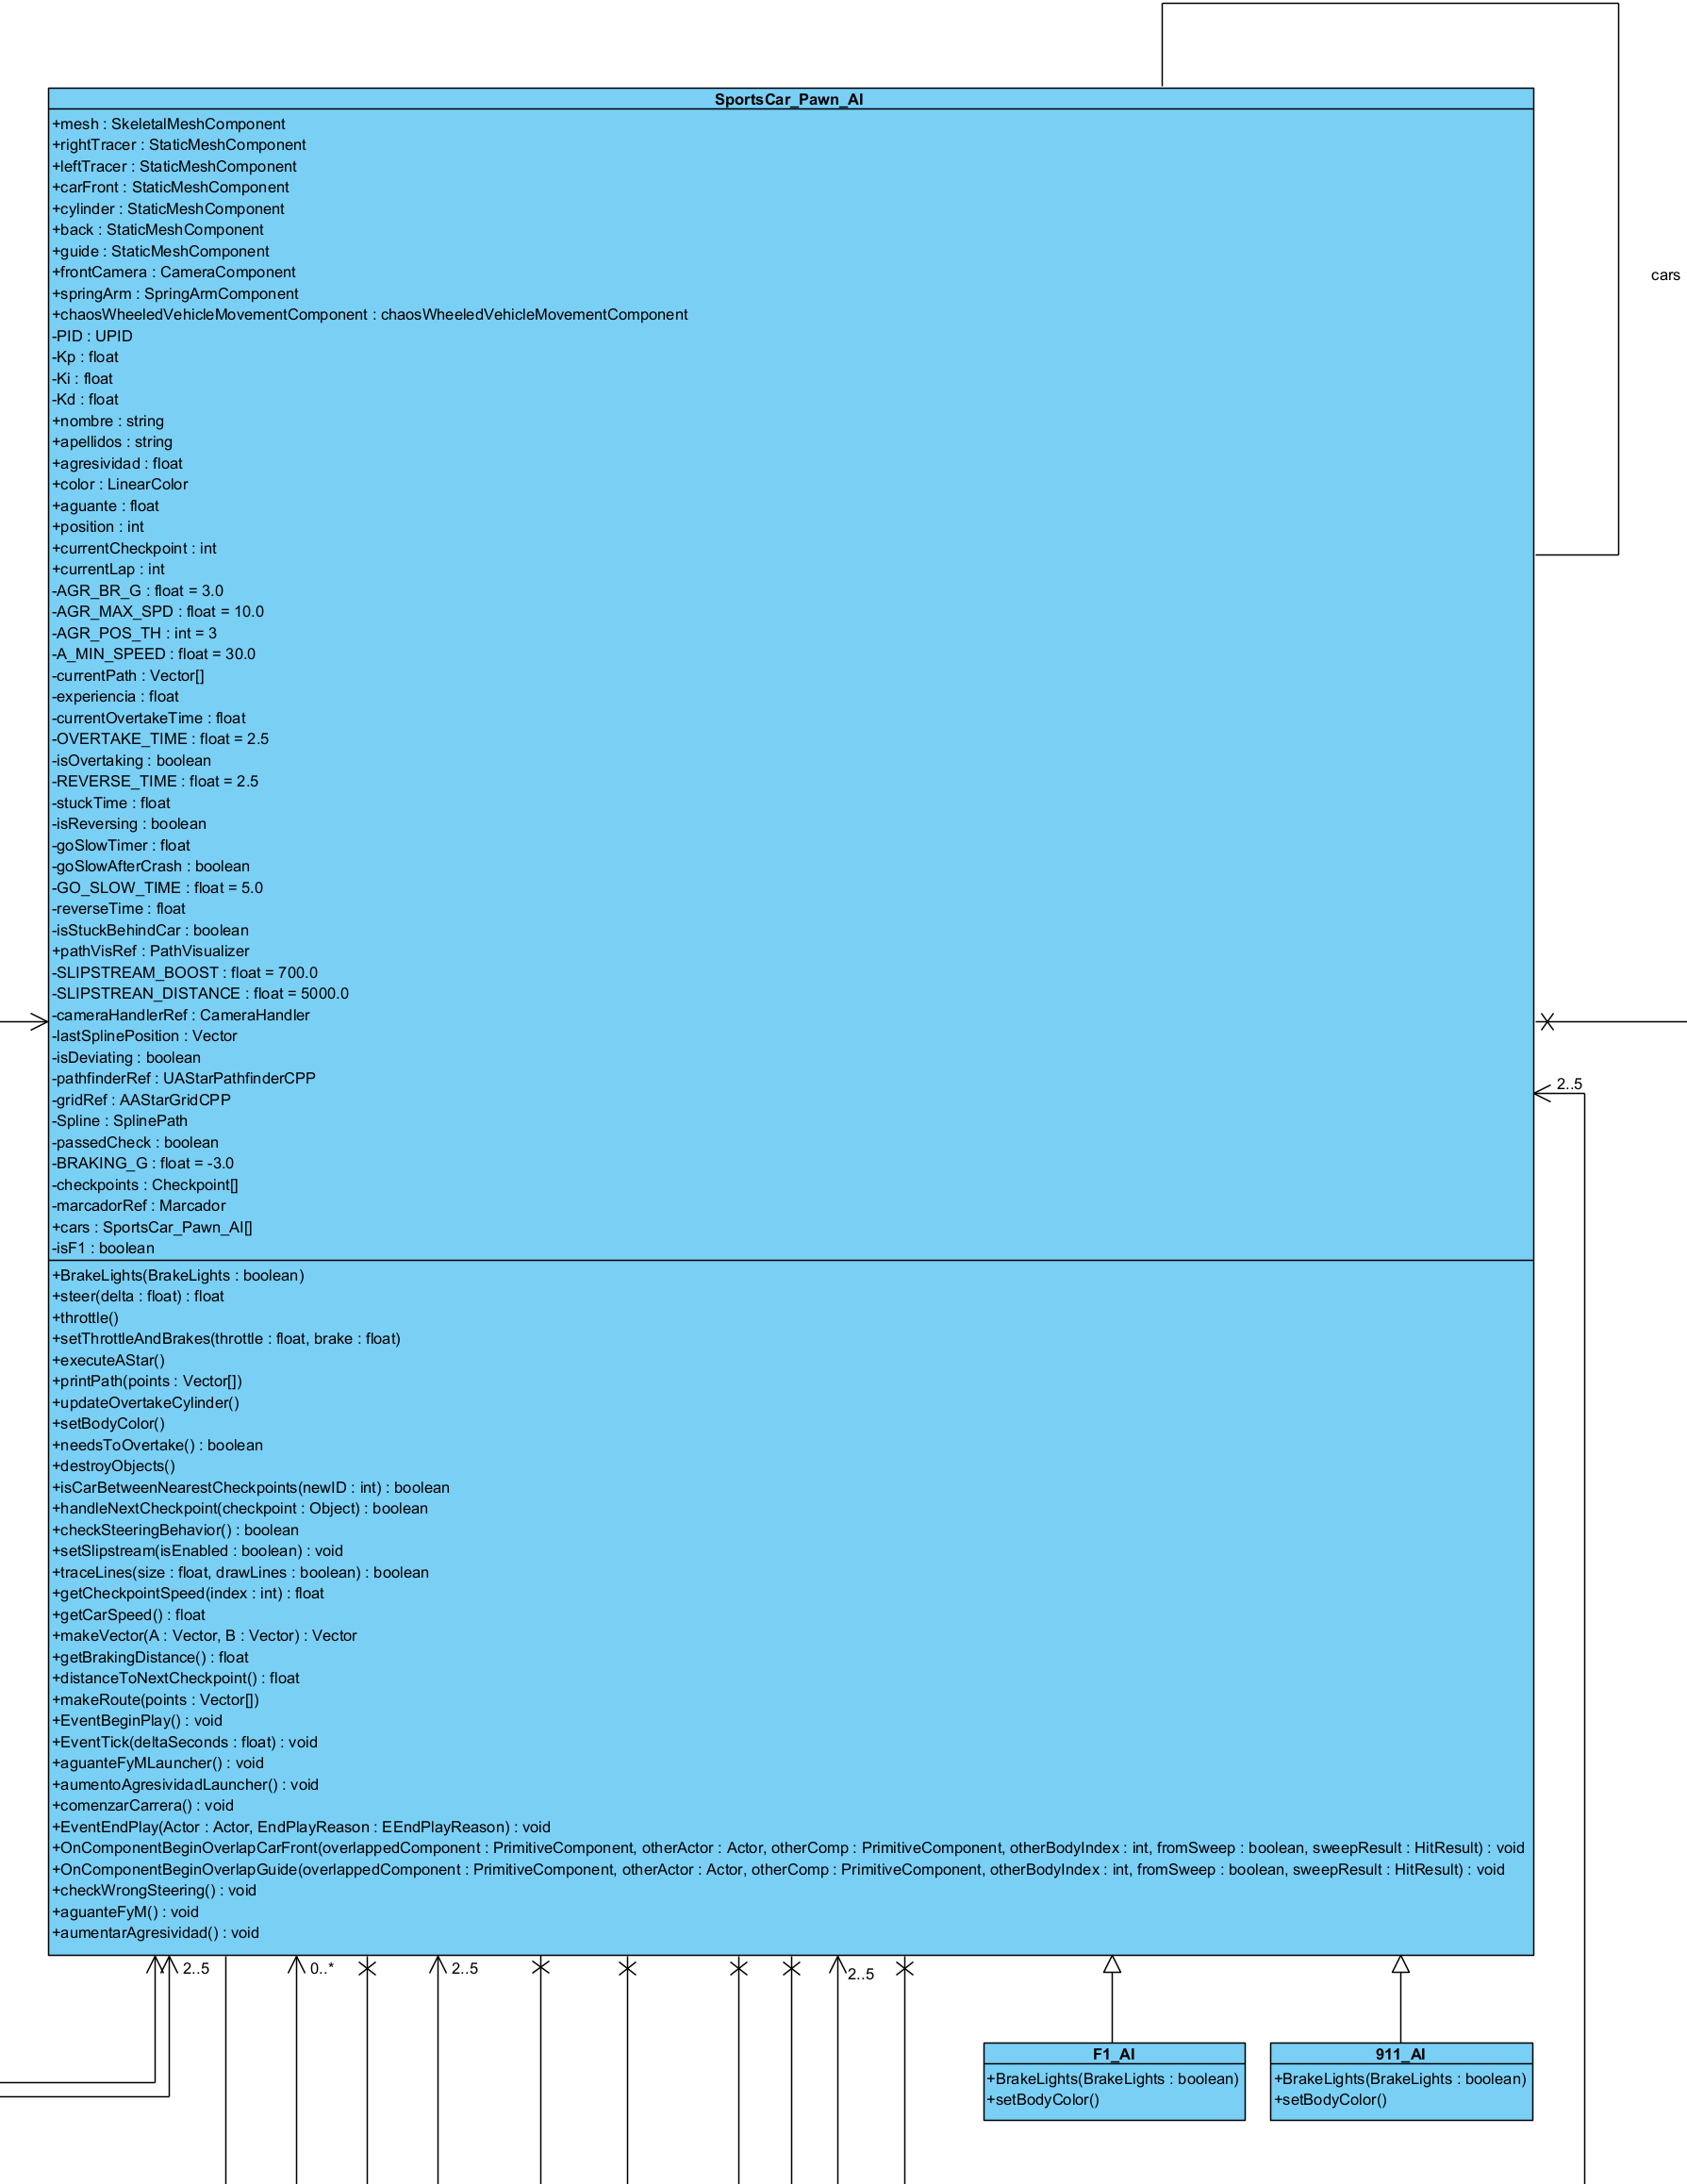
\includegraphics[width=\textwidth]{imagenes/classDiagram1.png}
    \caption{Primera sección del diagrama de clases.}
    \label{fig:class1}
\end{figure}


En la figura \ref{fig:class2}, aparece la clase padre de los coches del algoritmo genético, así como sus hijos. Además, se muestran las clases del controlador PID y el spline para las rutas, utilizados por los coches del algoritmo genético y los de la simulación. Por último, aparece el nivel del algoritmo genético, así como el bloque de meta ``TrainingStop'', el cambiador de spline ``ChangeSpline'', el objeto que crea la interfaz de usuario, la interfaz y la estructura utilizada para ejecutar el algoritmo.

\begin{figure}[H]
    \centering
    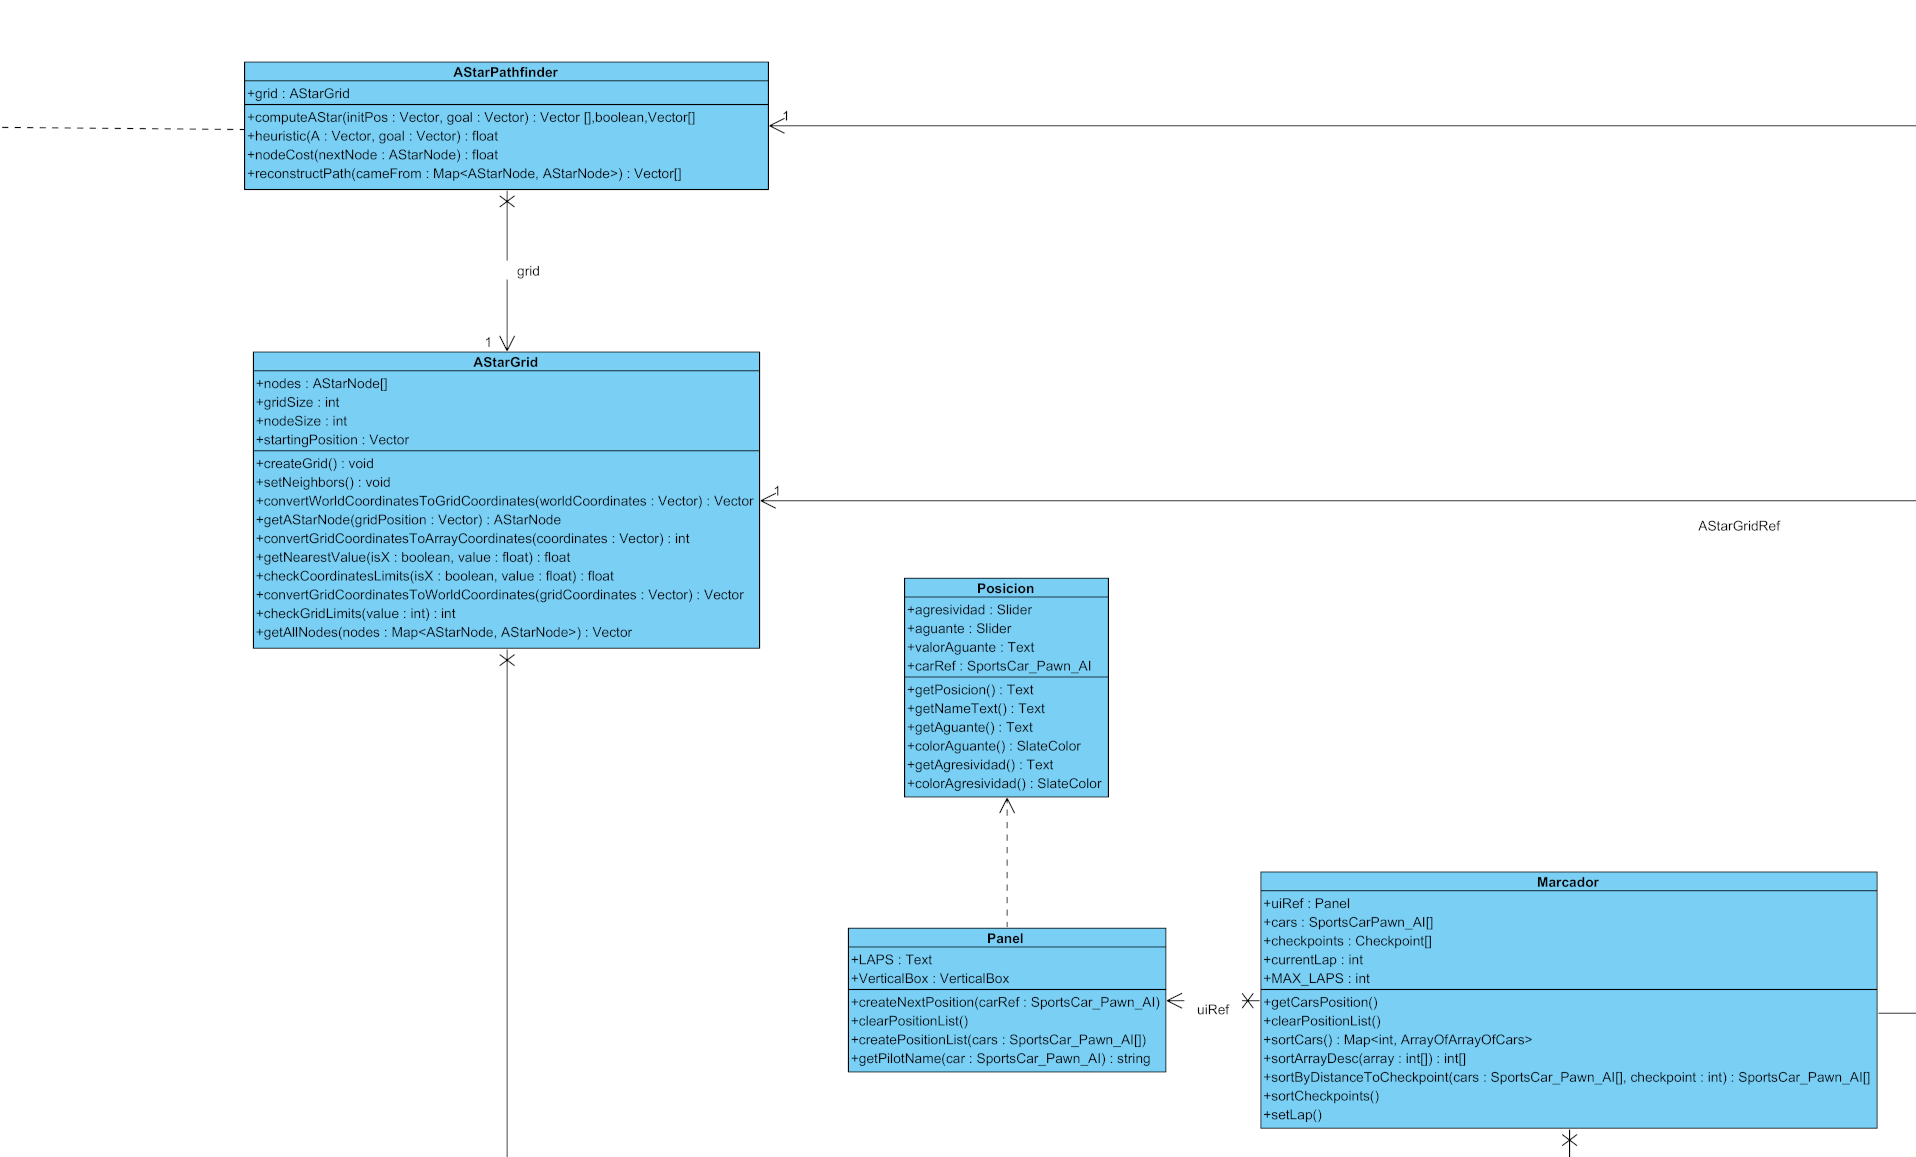
\includegraphics[width=\textwidth]{imagenes/classDiagram2.png}
    \caption{Segunda sección del diagrama de clases.}
    \label{fig:class2}
\end{figure}

En la figura \ref{fig:class3}, aparecen las clases relacionadas con la interfaz del configurador y el panel con las posiciones y la vuelta durante la carrera. También aparece la clase que gestiona las ventanas de diálogo y la instancia del juego ``VariablesMenu'' para pasar variables entre niveles.

\begin{figure}[H]
    \centering
    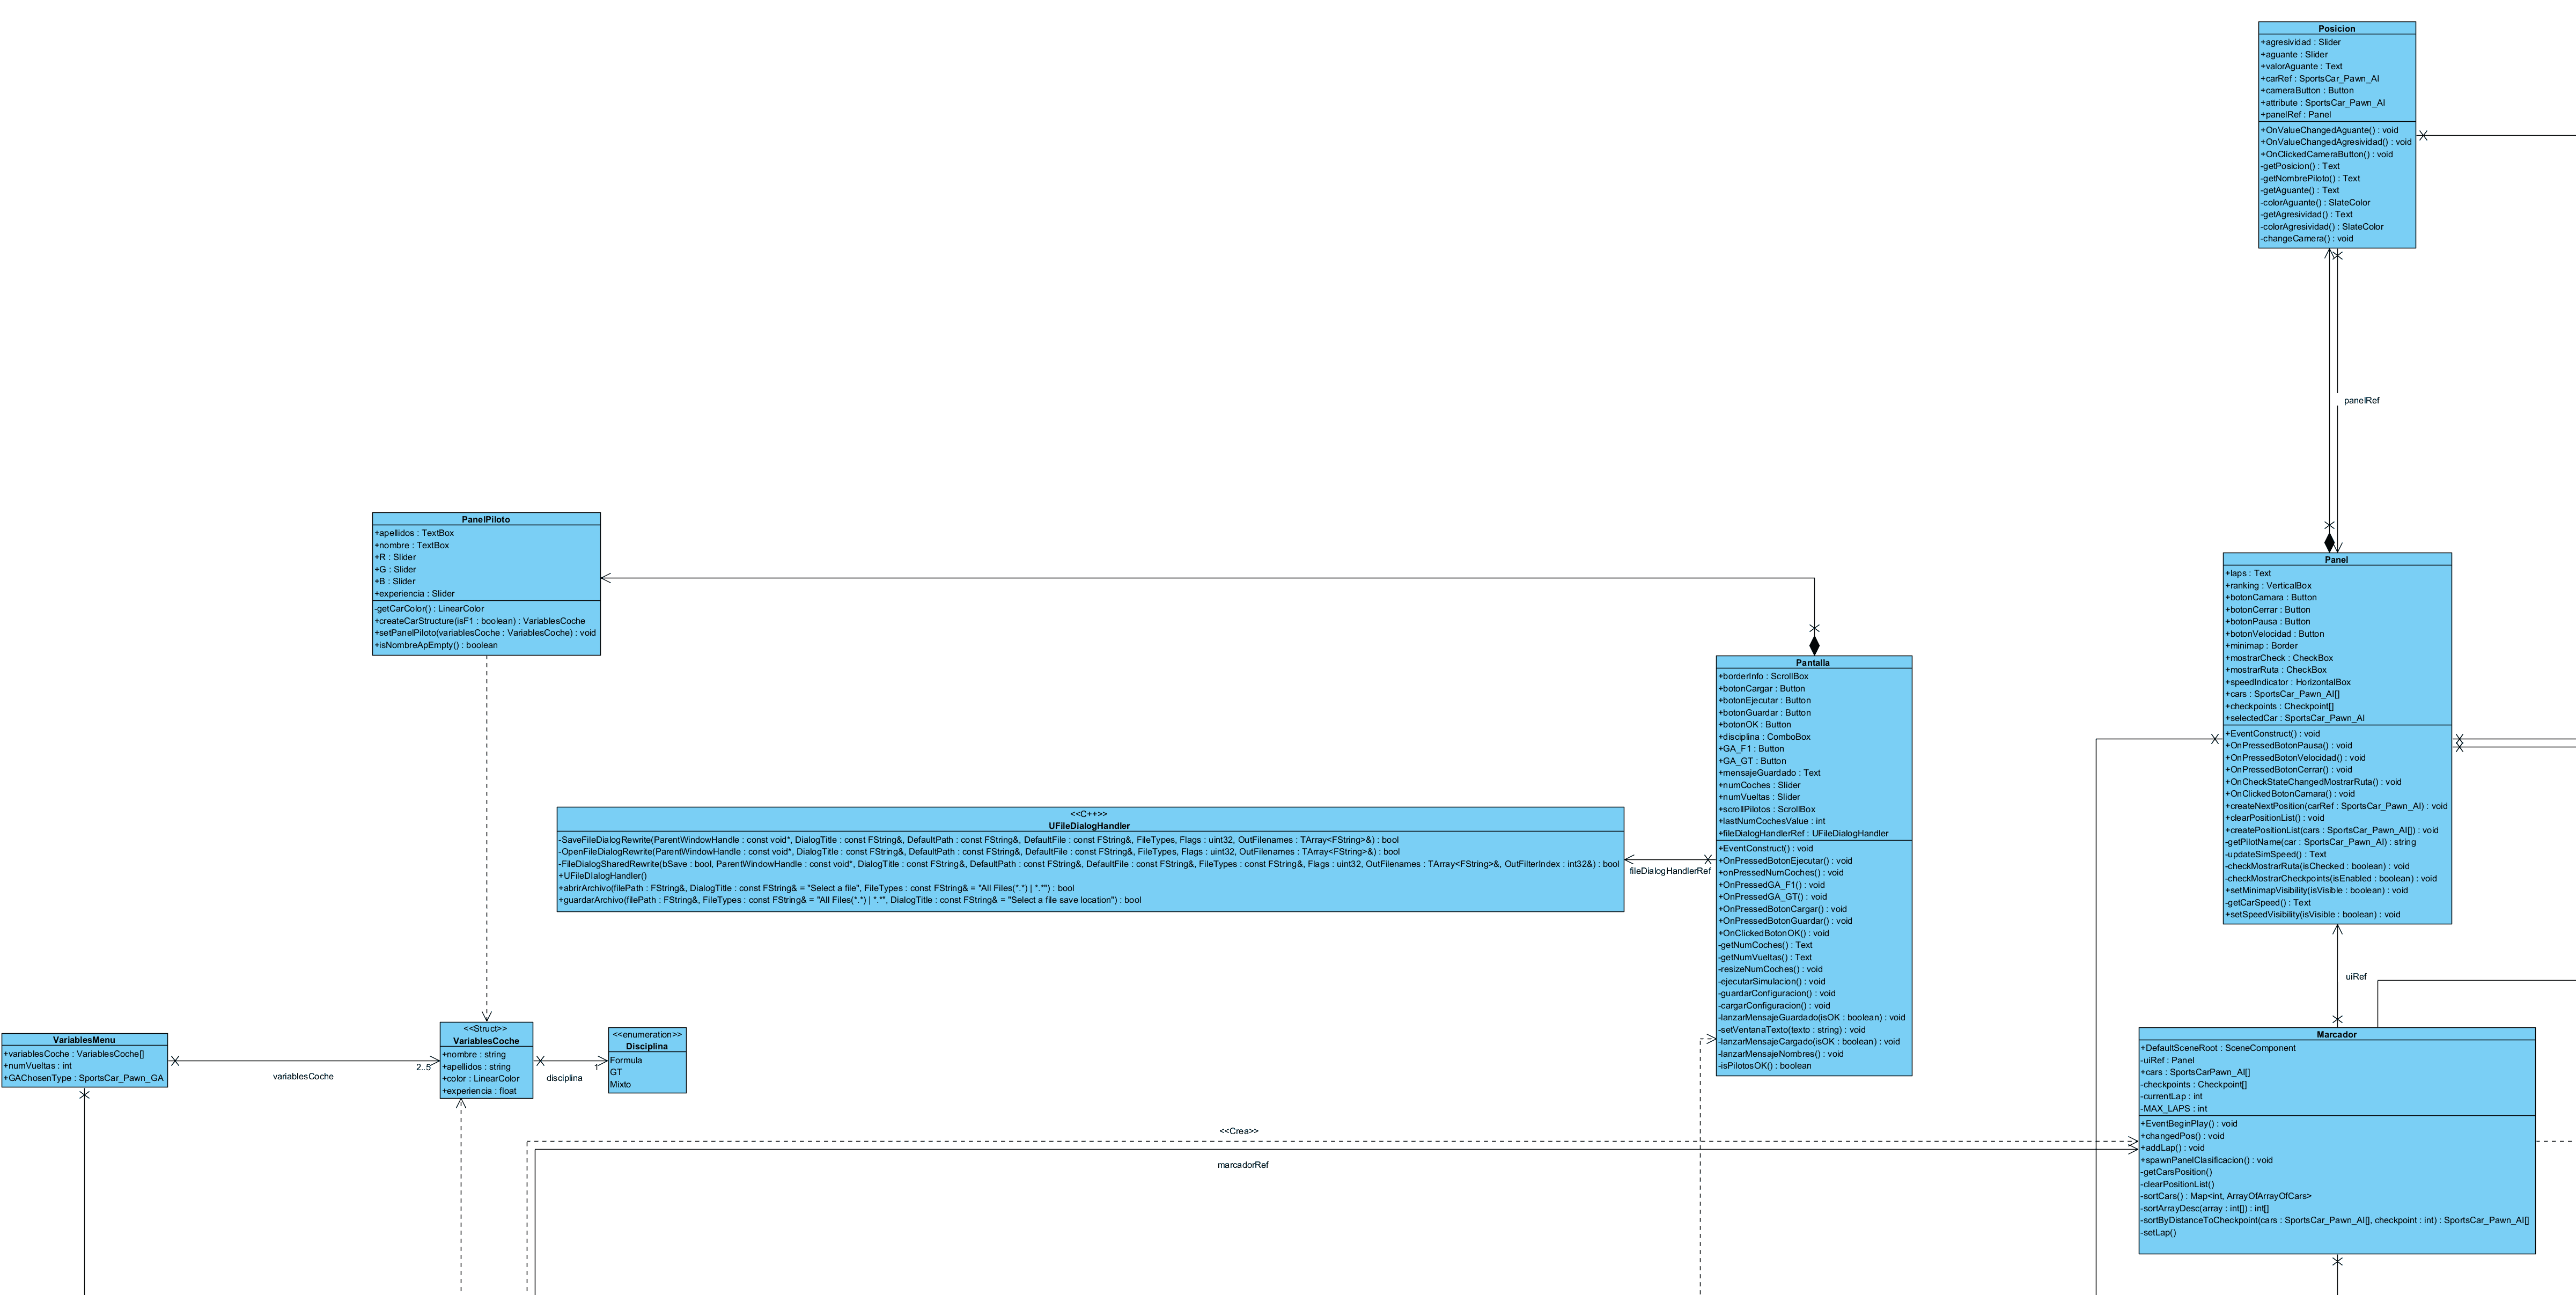
\includegraphics[width=\textwidth]{imagenes/classDiagram3.png}
    \caption{Tercera sección del diagrama de clases.}
    \label{fig:class3}
\end{figure}

En la figura \ref{fig:class4} se muestra la clase del nivel del circuito ``RacingLevel'', el nivel del configurador ``MenuLevel'', los puntos de generación de los coches en la parrilla, el gestor de la cámara para mantener el foco siempre, con independencia de la relación de aspecto, y los checkpoints.

\begin{figure}[H]
    \centering
    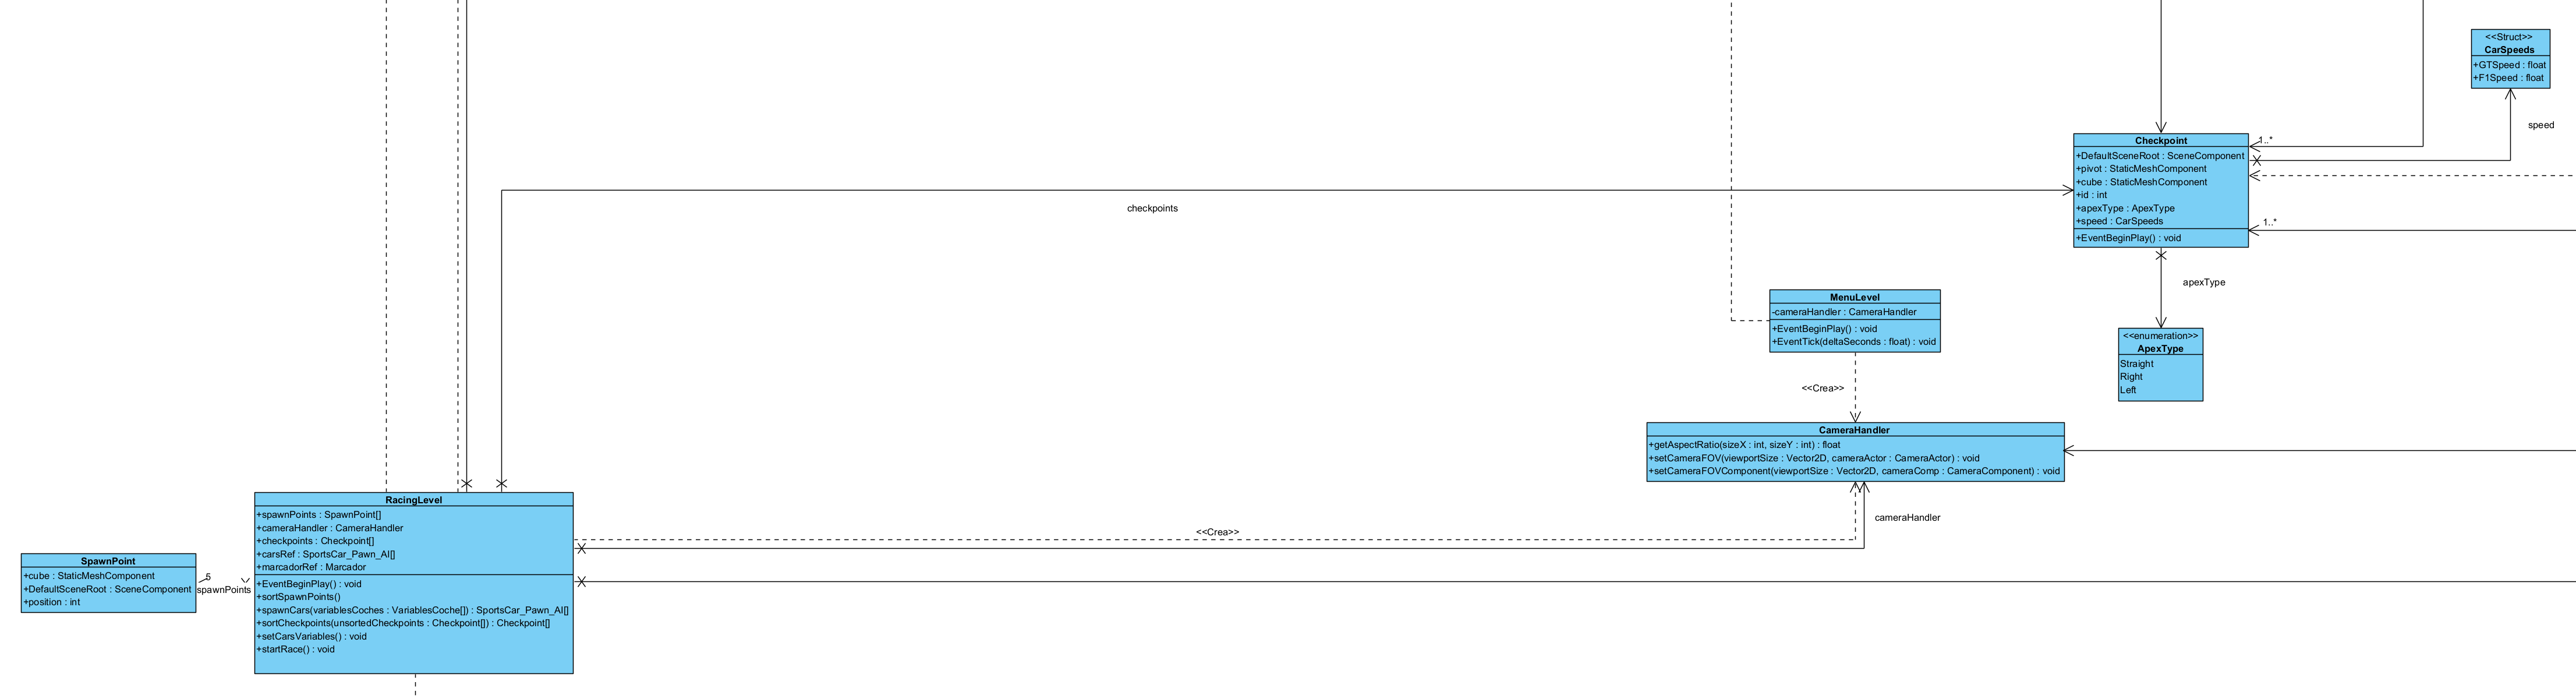
\includegraphics[width=\textwidth]{imagenes/classDiagram4.png}
    \caption{Cuarta sección del diagrama de clases.}
    \label{fig:class4}
\end{figure}

En esta última figura \ref{fig:class5}, aparecen las clases referentes al algoritmo de navegación, así como los nodos y los indicadores de límite de pista y ruta óptima. También aparece la clase generadora de la malla de navegación, el visualizador de rutas y la interfaz para la pantalla final al acabar la carrera.

\begin{figure}[H]
    \centering
    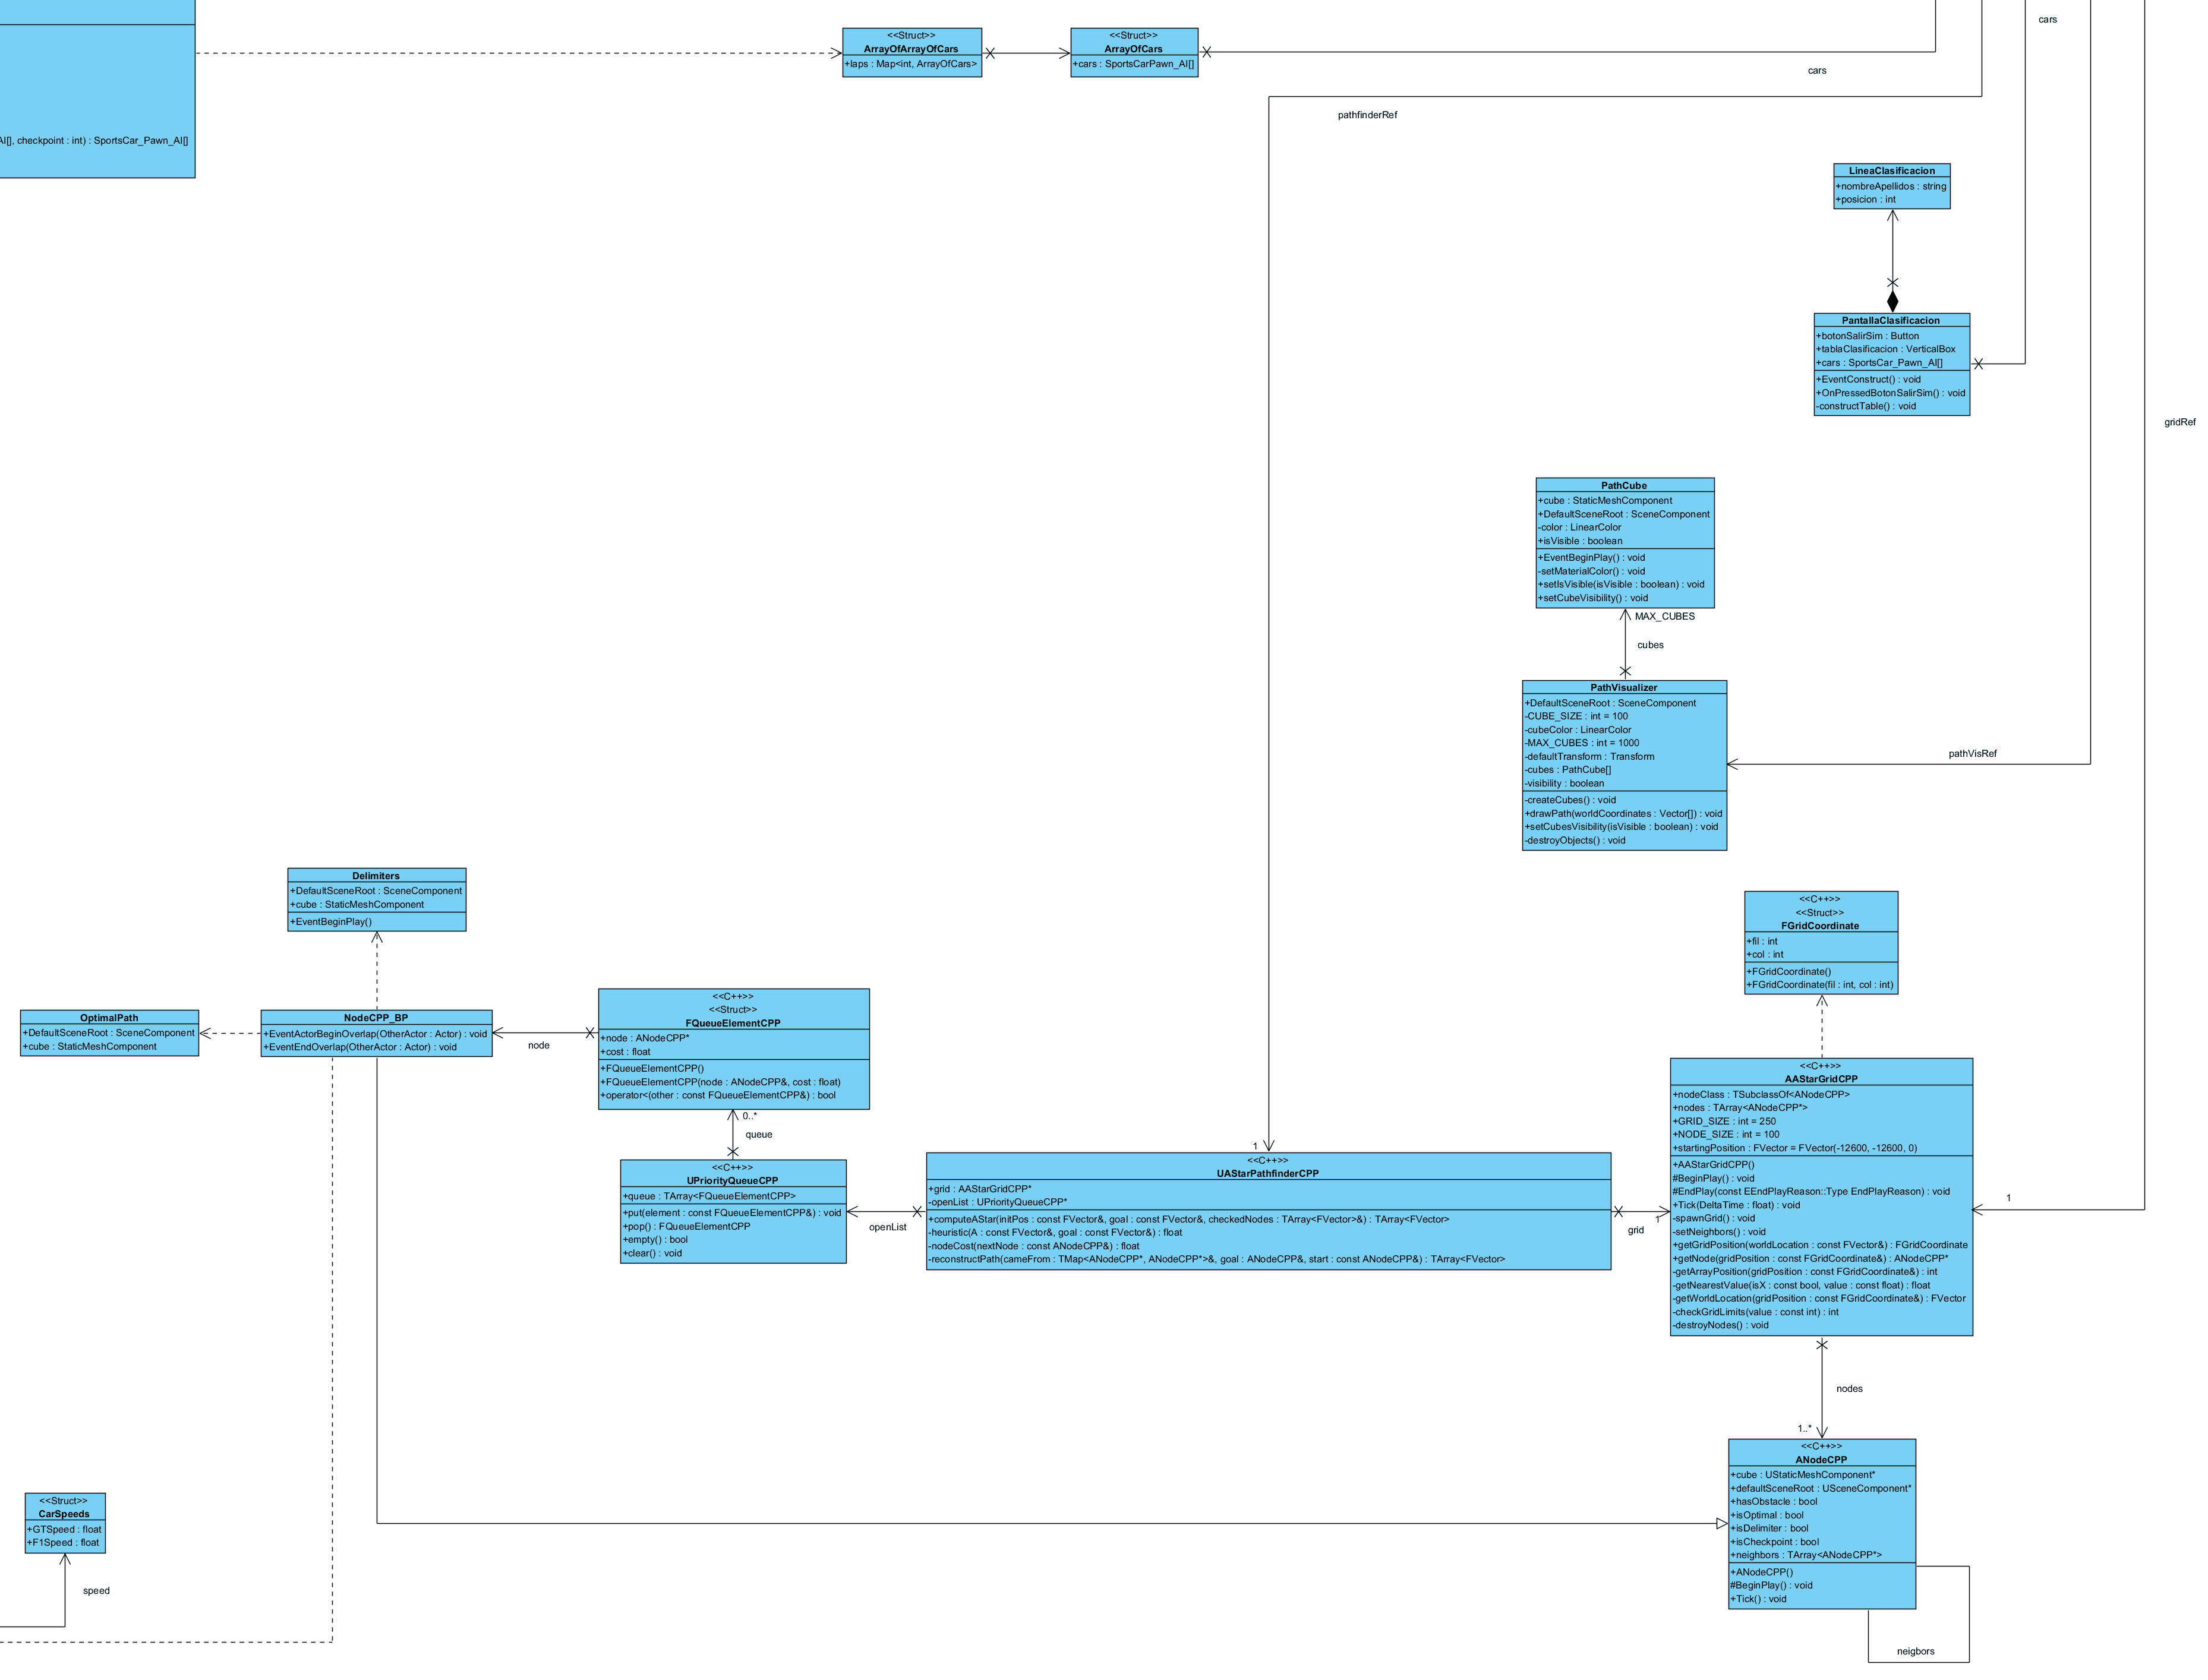
\includegraphics[width=\textwidth]{imagenes/classDiagram5.png}
    \caption{Quinta sección del diagrama de clases.}
    \label{fig:class5}
\end{figure}


\section{Diseño de la Interfaz de Usuario}

Los prototipos de las interfaces de usuario mencionadas a continuación se encuentran en la sección \ref{sec:proto-ui}.

\bigskip

La interfaz de usuario del configurador de la simulación
% (el prototipo se puede ver en la figura \ref{fig:protoconfig}) 
está dividida en dos secciones principales: a la izquierda se encuentra la sección para el número de vehículos y de pilotos, la disciplina y las opciones de importación y exportación de la configuración. A la derecha está la segunda sección, compuesta por las características de cada piloto, un menú desplegable para ejecutar el algoritmo genético y el botón para comenzar la simulación.

\begin{figure}[H]
    \centering
    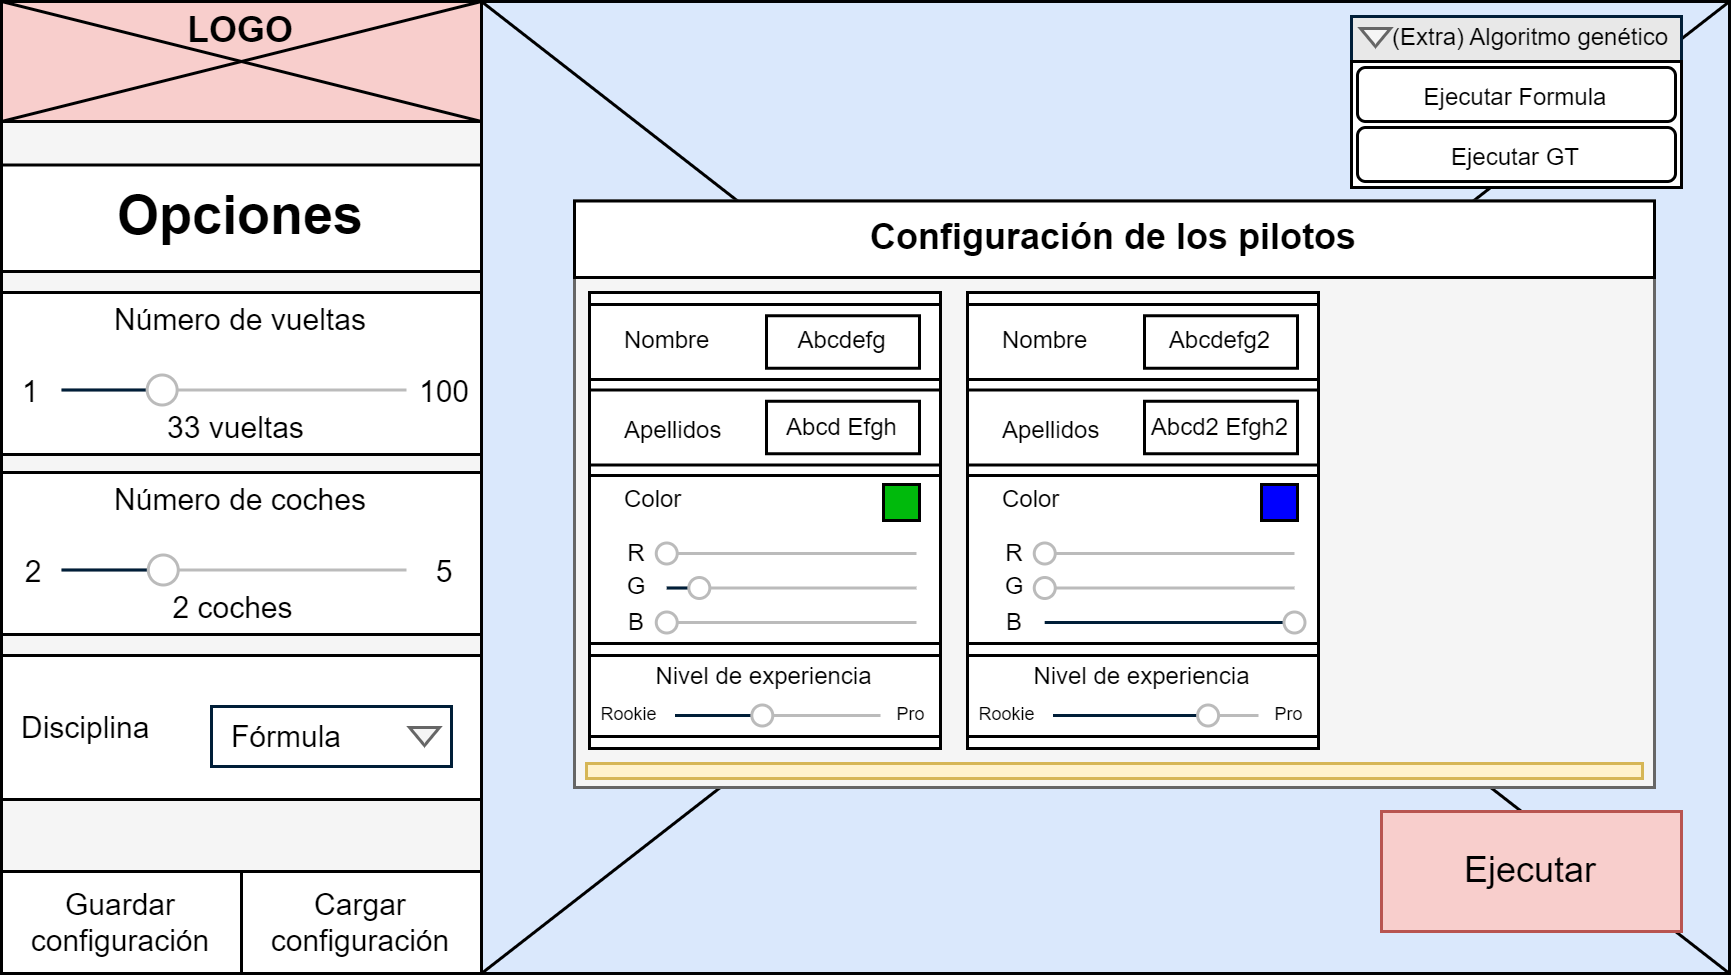
\includegraphics[width=\textwidth]{imagenes/pag1.png}
    \caption{Interfaz del configurador antes de la carrera.}
\end{figure}

Durante la carrera, se mostrará un listado de posiciones de los pilotos y un contador de vueltas 
% (prototipo en la figura \ref{fig:protoranking}) 
en la parte izquierda de la pantalla. Este listado permitirá visualizar y modificar el estado de cada piloto en tiempo real. La disposición de los elementos será similar a la de disciplinas como la Fórmula 1, donde el ranking de pilotos y el contador de vueltas aparecen a la izquierda, y en cada celda de posición aparecen las tres primeras letras del apellido. En este proyecto, he decidido añadir también la primera letra del nombre, en caso de que haya varios pilotos con el mismo apellido. Además, aparecerá a la derecha un menú desplegable con las opciones de visualización de ruta y de los checkpoints.


\begin{figure}[H]
    \centering
    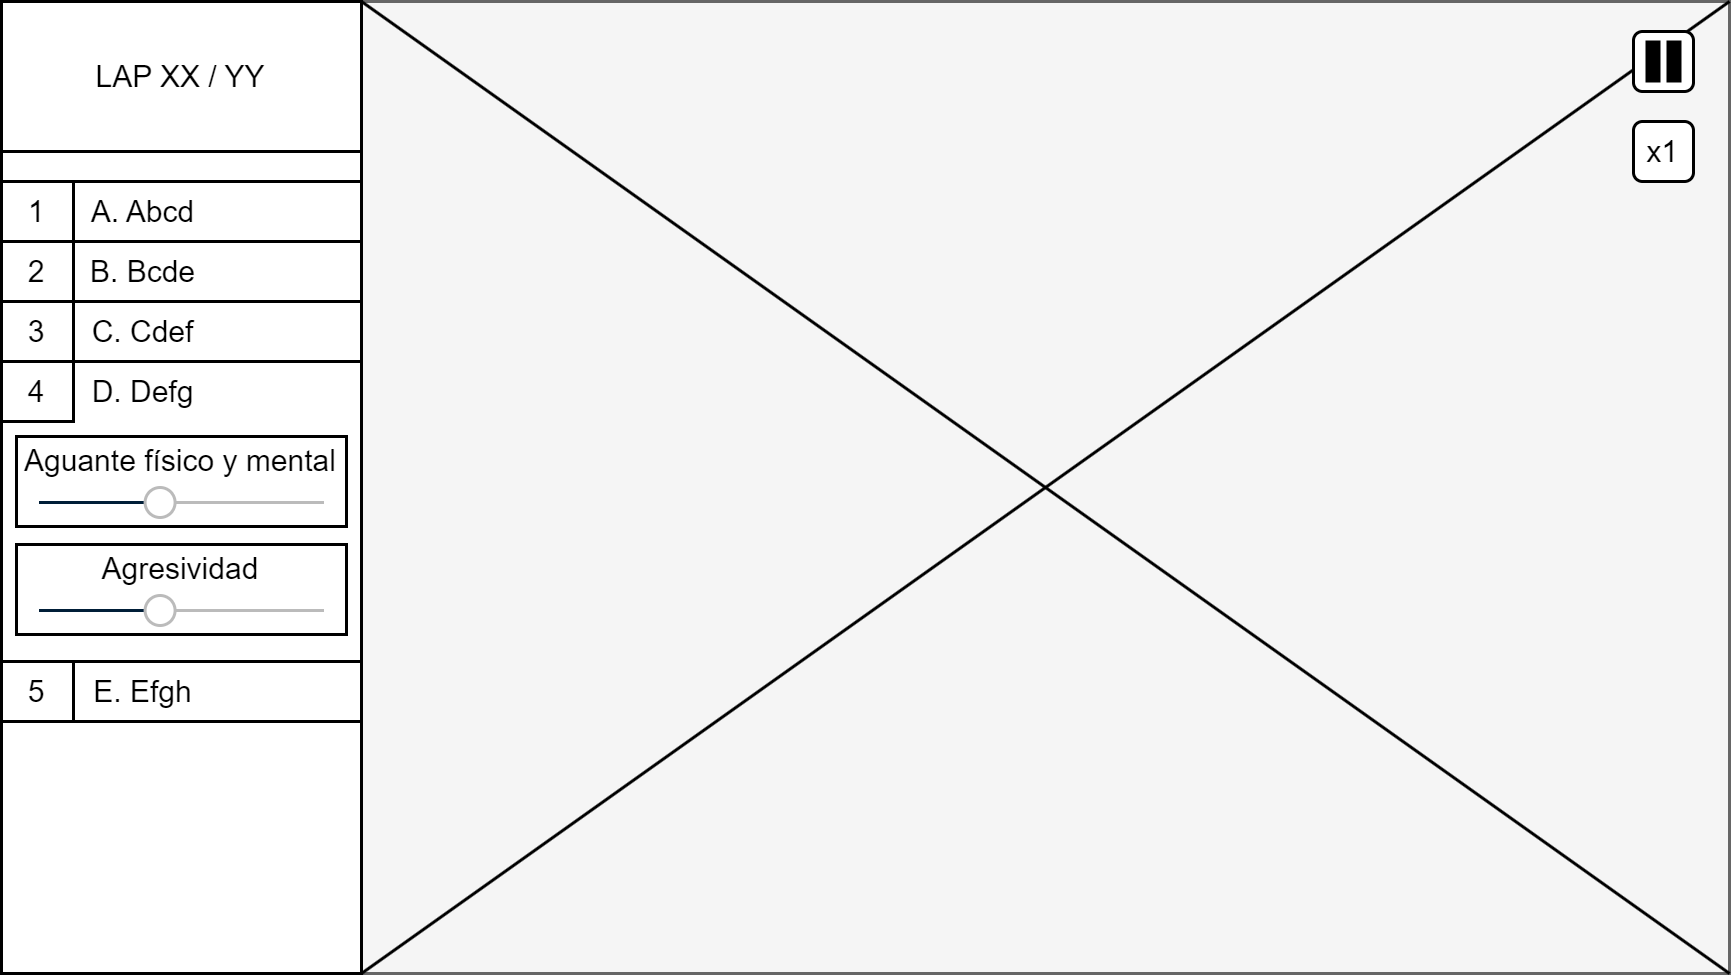
\includegraphics[width=\textwidth]{imagenes/pag2.png}
    \caption{Interfaz de las opciones durante la carrera.}
    \label{fig:boc-ui-race}
\end{figure}

Al finalizar la carrera, aparecerá un listado de posiciones con los nombres de los pilotos, así como un botón para salir de la simulación al configurador de carrera.

\begin{figure}[H]
    \centering
    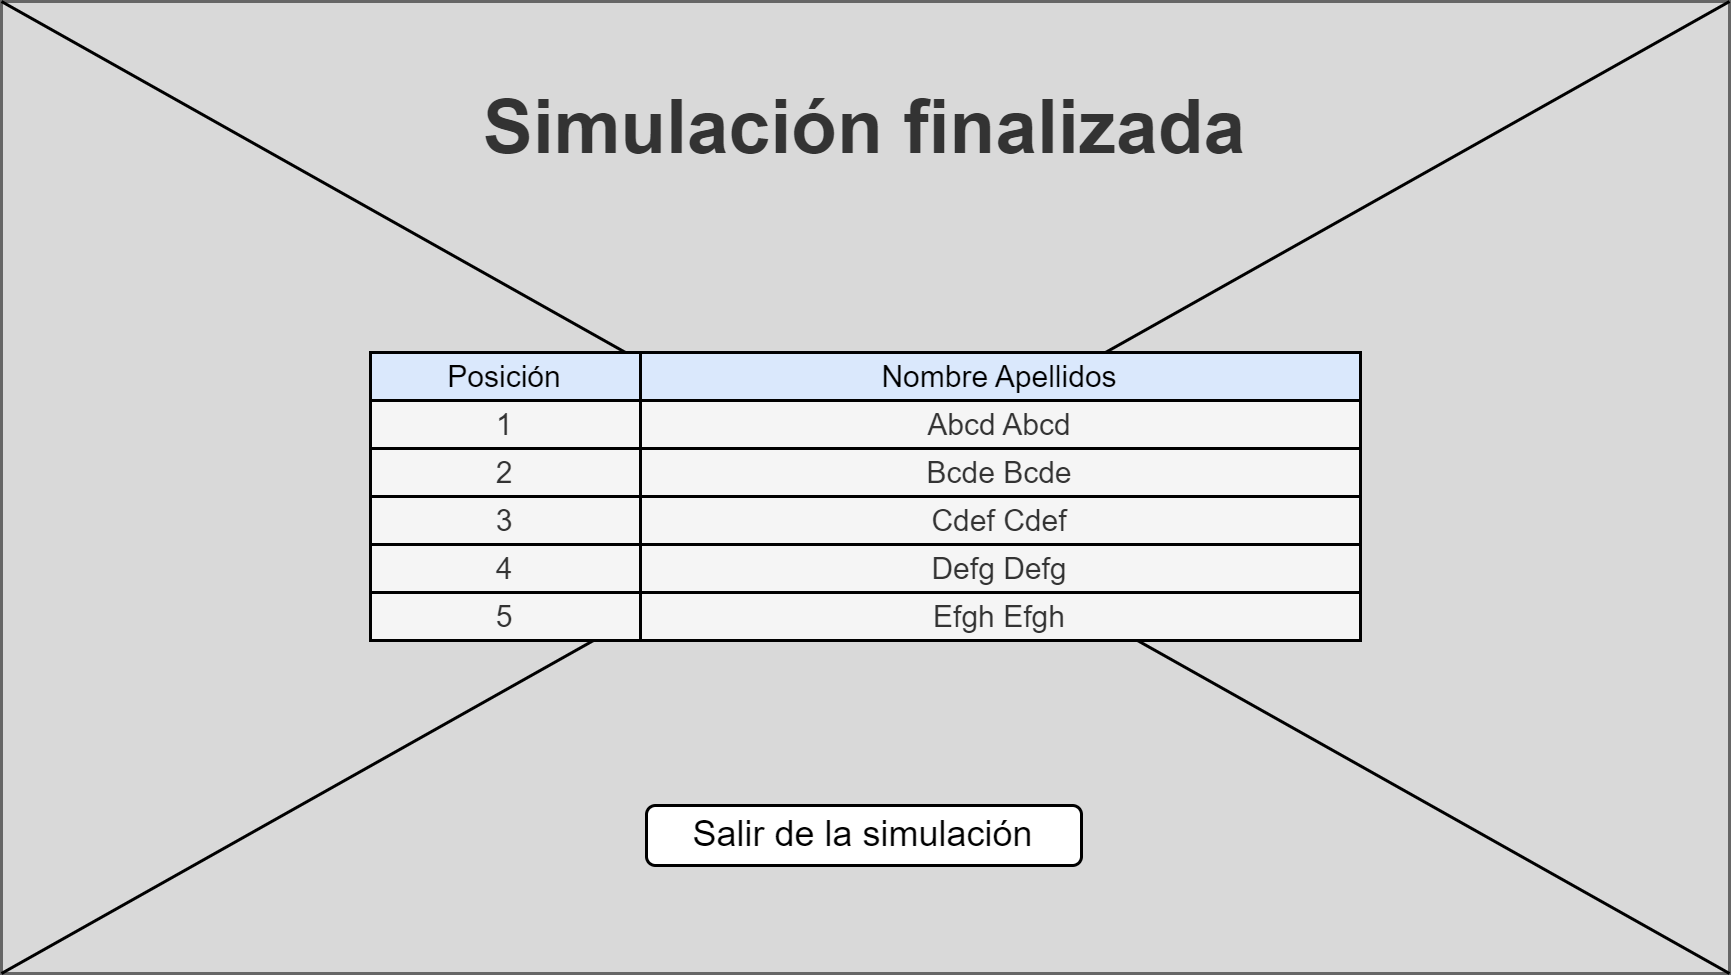
\includegraphics[width=\textwidth]{imagenes/pantallafinal.png}
    \caption{Interfaz de los resultados al salir de la carrera.}
    \label{fig:resultados-sim}
\end{figure}

\newpage

Por último, la interfaz del algoritmo genético está compuesta por una tabla con los 10 mejores valores para las constantes del PID (implementación y explicación en la sección \ref{sec:pid-sec}) y un botón para cerrar la ejecución del algoritmo genético y volver al configurador de carreras.

\begin{figure}[H]
    \centering
    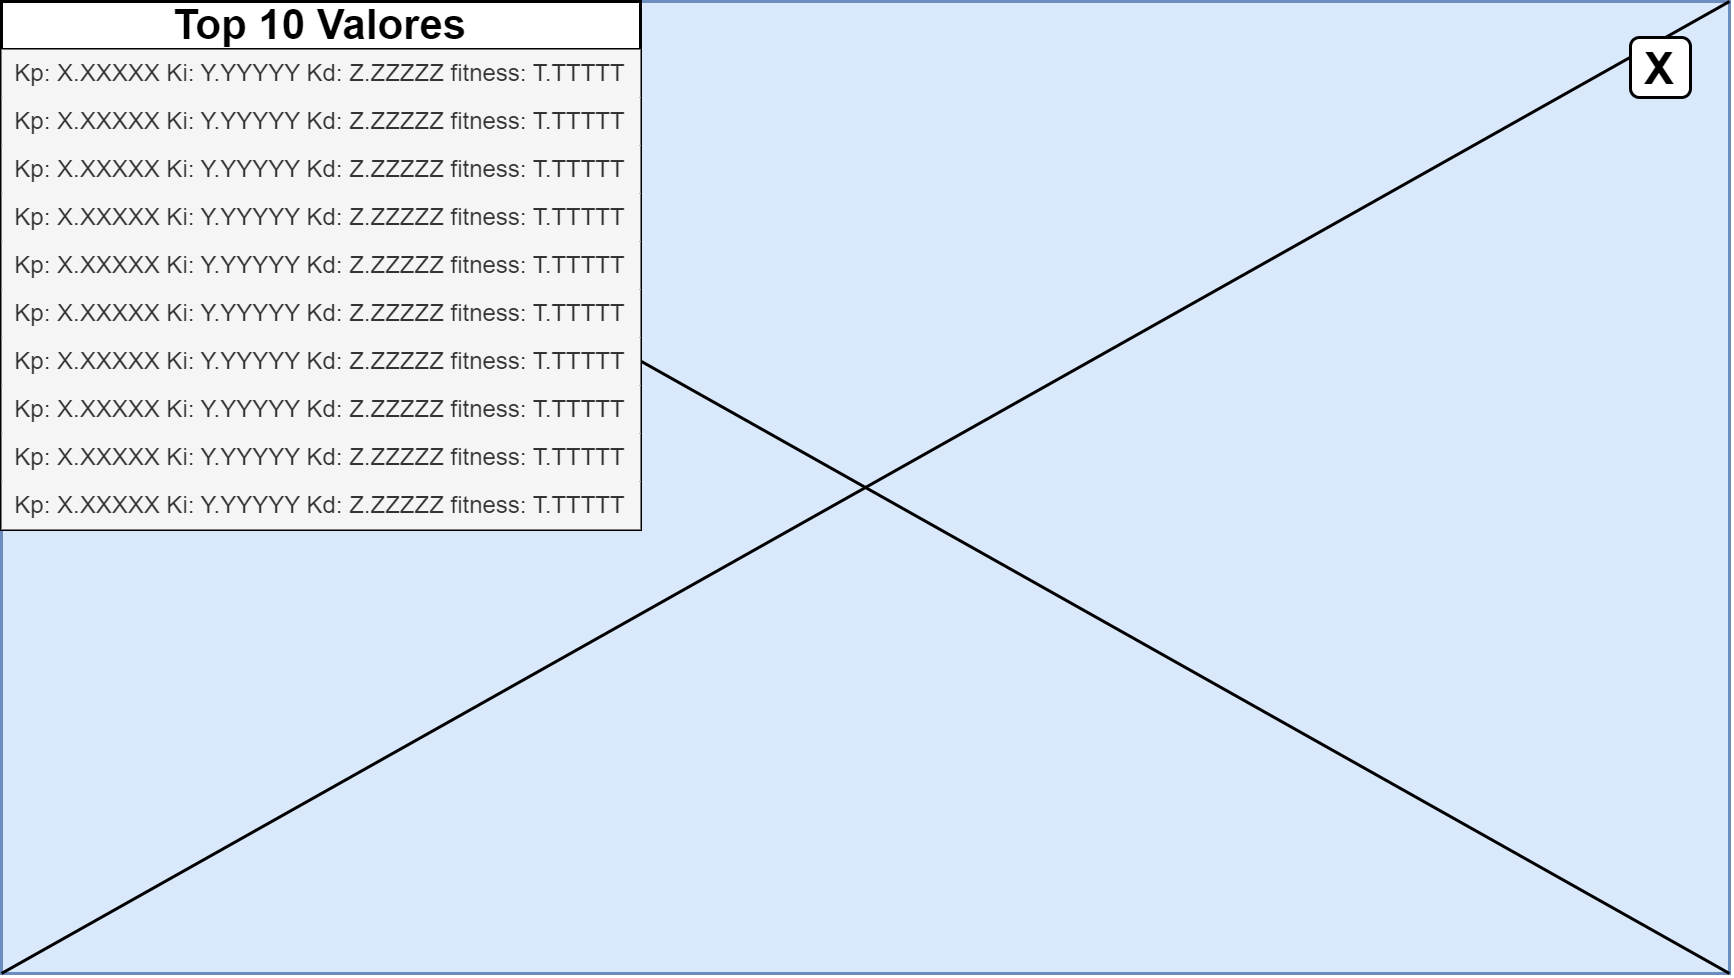
\includegraphics[width=\textwidth]{imagenes/ga.png}
    \caption{Interfaz de la ejecución del algoritmo genético.}
\end{figure}

\newpage

\section{Diagrama de navegación}

% La navegación por la interfaz de usuario en la aplicación es relativamente sencilla, al estar formada por dos pantallas: el configurador de simulación y la carrera en curso.

% \bigskip

El diagrama de navegación de la aplicación es el siguiente:

% foto del diagrama de navegacion
\begin{figure}[H]
    \centering
    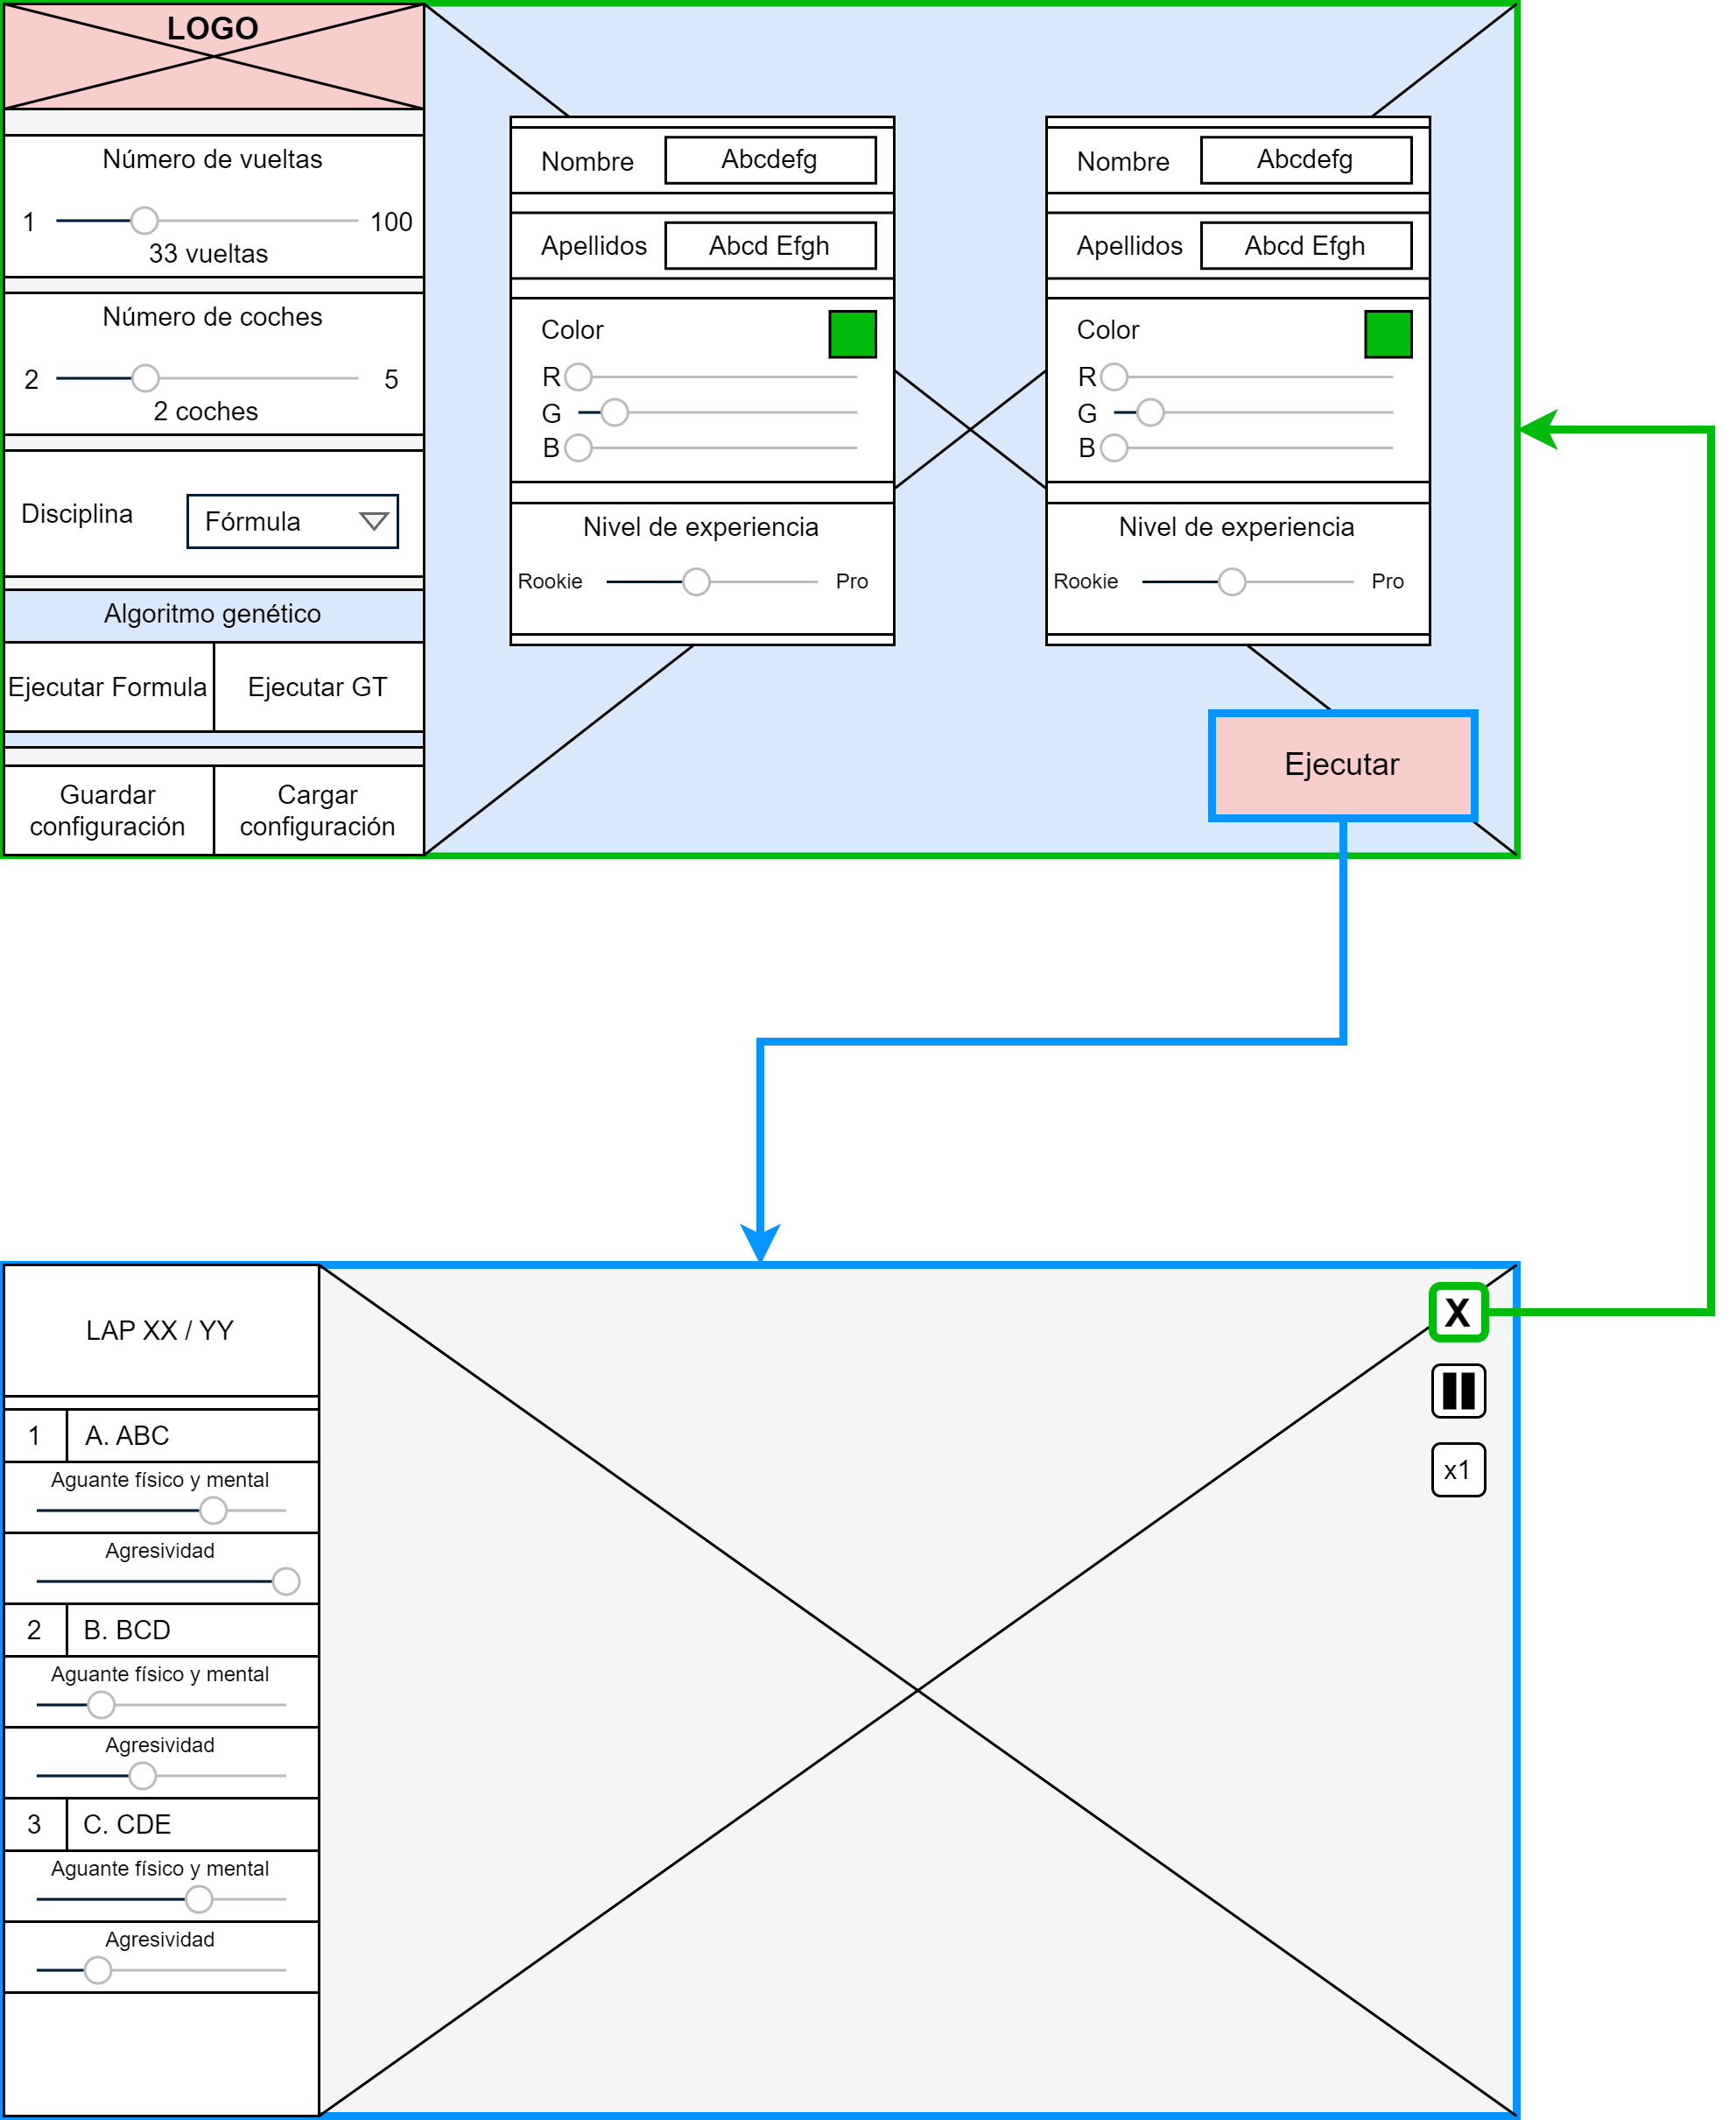
\includegraphics[width=\textwidth]{imagenes/nav.png}
    \caption{Diagrama de navegación de la interfaz de usuario de la aplicación.}
\end{figure}

Como se puede observar, desde el configurador hay dos posibles pantallas siguientes: la carrera y el algoritmo genético. Si se pulsa sobre el botón de ejecutar, dará comienzo a la carrera, y al terminar aparecerá automáticamente la siguiente pantalla con las posiciones finales de los pilotos. En esta pantalla solo es posible elegir la opción de volver al configurador. 

\bigskip

En la ejecución del algoritmo genético y durante la carrera, antes de que acabe, se podrá pulsar el botón con el símbolo ``X'' para salir de nuevo al configurador.

\bigskip

Por último, cuando todos los coches cruzan la línea de meta, aparecerá una pantalla con los resultados y un botón que si se pulsa lleva de nuevo al configurador.

% Como se puede observar en el diagrama de navegación, al pulsar el botón de ejecutar aparecerá la nueva pantalla para ejecutar la simulación y dar comienzo a la carrera. Asimismo, si se pulsa el botón con el símbolo ``X'', se cerrará la simulación en curso y aparecerá de nuevo el configurador.
